\documentclass[aspectratio=169,12pt]{beamer}

% =========================================================
% THEME
% =========================================================

\usetheme{Madrid}

% =========================================================
% PACKAGES
% =========================================================

\usepackage{amsmath}
\usepackage{amssymb}
\usepackage{booktabs}
\usepackage{array}
\usepackage{graphicx}
\usepackage{tikz}

\usetikzlibrary{arrows.meta, positioning, shapes.geometric}

% =========================================================
% PASTEL PROFESSIONAL COLORS
% =========================================================

\definecolor{PastelBlue}{RGB}{91,135,166}
\definecolor{PastelLavender}{RGB}{125,118,155}
\definecolor{LightBlue}{RGB}{235,242,247}
\definecolor{LightLavender}{RGB}{242,240,247}
\definecolor{DarkText}{RGB}{55,65,75}

\setbeamercolor{structure}{fg=PastelBlue}

\setbeamercolor{normal text}{
    fg=DarkText,
    bg=white
}

\setbeamercolor{frametitle}{
    fg=PastelBlue,
    bg=LightBlue
}

\setbeamercolor{block title}{
    fg=white,
    bg=PastelBlue
}

\setbeamercolor{block body}{
    fg=DarkText,
    bg=LightBlue
}

\setbeamercolor{block title example}{
    fg=white,
    bg=PastelLavender
}

\setbeamercolor{block body example}{
    fg=DarkText,
    bg=LightLavender
}

% =========================================================
% FOOTER
% =========================================================

% Show author, title and date only
\setbeamertemplate{footline}
{
    \leavevmode%
    \hbox{%
        \begin{beamercolorbox}[
            wd=.33\paperwidth,
            ht=2.5ex,
            dp=1.125ex,
            leftskip=.3cm
        ]{author in head/foot}
            \usebeamerfont{author in head/foot}\insertshortauthor
        \end{beamercolorbox}%
        \begin{beamercolorbox}[
            wd=.34\paperwidth,
            ht=2.5ex,
            dp=1.125ex,
            center
        ]{title in head/foot}
            \usebeamerfont{title in head/foot}\insertshorttitle
        \end{beamercolorbox}%
        \begin{beamercolorbox}[
            wd=.33\paperwidth,
            ht=2.5ex,
            dp=1.125ex,
            rightskip=.3cm
        ]{date in head/foot}
            \usebeamerfont{date in head/foot}
            \hfill\insertshortdate\hspace{0.2cm}
        \end{beamercolorbox}%
    }%
    \vskip0pt%
}

% Remove navigation symbols
\setbeamertemplate{navigation symbols}{}

% =========================================================
% DOCUMENT INFORMATION
% =========================================================

\title{Descriptive Statistics}
\subtitle{Mathematics for Computing -- Module 3}

% Short author name used in the footer
\author[Arya T S]{Arya T S}

% Full institute information shown on the title page
\institute{
    M.Tech Artificial Intelligence \& Software Engineering\\
    Cochin University of Science and Technology (CUSAT)
}

\date{September 2026}

% =========================================================
% DOCUMENT
% =========================================================

\begin{document}

% =========================================================
% TITLE SLIDE
% =========================================================

% \begin{frame}[plain]
%     \titlepage
% \end{frame}

% =========================================================
% MODULE OVERVIEW -- SLIDE 1
% =========================================================

\begin{frame}{Module Overview}

\begin{columns}[T,totalwidth=\textwidth]

% ---------- LEFT COLUMN ----------
\begin{column}{0.48\textwidth}

\begin{block}{Part I -- Foundations}

\begin{itemize}
    \item Statistics
    \item Data
    \item Information
    \item Knowledge
    \item Intelligence
    \item Types of Data
\end{itemize}

\end{block}

\end{column}

% ---------- RIGHT COLUMN ----------
\begin{column}{0.48\textwidth}

\begin{block}{Part II -- Descriptive Statistics}

\begin{itemize}
    \item Measures of Central Tendency
    \item Measures of Dispersion
    \item Histogram
    \item Box Plot
    \item Outliers
    \item Skewness
    \item Kurtosis
\end{itemize}

\end{block}

\end{column}

\end{columns}

\end{frame}

% =========================================================
% MODULE OVERVIEW -- SLIDE 2
% =========================================================

\begin{frame}{Module Overview}

\begin{columns}[T,totalwidth=\textwidth]

% ---------- LEFT COLUMN ----------
\begin{column}{0.48\textwidth}

\begin{block}{Part III -- Sample Statistics}

\begin{itemize}
    \item Population and Sample
    \item Sample Mean
    \item Sample Variance
    \item Order Statistics
    \item Covariance
    \item Sample Covariance
    \item Correlation
    \item Sample Covariance Matrix
\end{itemize}

\end{block}

\end{column}

% ---------- RIGHT COLUMN ----------
\begin{column}{0.48\textwidth}

\begin{block}{Part IV -- Frequentist Statistics}

\begin{itemize}
    \item Frequentist Statistics
    \item Sampling
    \item Sampling Distribution
    \item Standard Error
    \item Estimator, Estimate and Parameter
    \item Bias and Variance
    \item Mean Square Error
    \item Consistency
    \item Central Limit Theorem, Confidence Intervals
\end{itemize}

\end{block}

\end{column}

\end{columns}

\end{frame}

% =========================================================
% MODULE OVERVIEW -- SLIDE 3
% =========================================================

\begin{frame}{Module Overview}

\begin{columns}[T,totalwidth=\textwidth]

% ---------- LEFT COLUMN ----------
\begin{column}{0.48\textwidth}

\begin{block}{Part V -- Model Estimation}

\begin{itemize}
    \item Parametric Model Estimation
    \item Maximum Likelihood Estimation
    \item Non-parametric Model Estimation
    \item Empirical CDF
    \item Kernel Density Estimation
    \item Parametric vs Non-parametric Comparison
\end{itemize}

\end{block}

\end{column}

% ---------- RIGHT COLUMN ----------
\begin{column}{0.48\textwidth}

\begin{block}{Final}

\begin{itemize}
    \item Applications in Computing and AI
    \item Conclusion
    \item References
\end{itemize}

\end{block}

\end{column}

\end{columns}

\end{frame}

% =========================================================
% CONTENT FILES
% =========================================================

% =========================================================
% PART I -- FOUNDATIONS
% =========================================================

\section{Foundations}

% ---------------------------------------------------------
% 1. STATISTICS
% ---------------------------------------------------------

\begin{frame}{1. Statistics}

\textbf{Definition}

Statistics is the science of collecting, organizing, summarizing,
analyzing, interpreting, and presenting data to obtain meaningful
information and support decision-making.

\vspace{0.4cm}

\textbf{Main branches}

\begin{itemize}
    \item \textbf{Descriptive Statistics} -- summarizes and presents data.
    \item \textbf{Inferential Statistics} -- uses sample data to draw
    conclusions about a population.
\end{itemize}

\vspace{0.3cm}

\textbf{Example}

For the marks of 50 students, calculating the mean and standard
deviation describes the data, while using the sample to estimate
the average marks of the entire class is an inferential task.

\end{frame}


% ---------------------------------------------------------
% 2. DATA
% ---------------------------------------------------------

\begin{frame}{2. Data}

\textbf{Definition}

Data are raw facts, observations, measurements, or values collected
for analysis.

\textbf{Examples}

\begin{itemize}
    \item Student marks: $72, 85, 64, 91$
    \item Age: $20, 21, 22, 20$
    \item Temperature: $28.5^\circ C$
    \item Image pixels represented by numerical values
\end{itemize}

\textbf{Mathematical Representation}

A dataset can be represented as

\[
X = \{x_1,x_2,\ldots,x_n\}
\]

where $x_i$ represents an observation and $n$ is the number of
observations.

\textbf{Application:} Data forms the basic input for statistical
analysis and machine learning models.

\end{frame}


% ---------------------------------------------------------
% 3. INFORMATION
% ---------------------------------------------------------

\begin{frame}{3. Information}

\textbf{Definition}

Information is processed, organized, and interpreted data that
provides meaning.

\textbf{Example}

Suppose the marks are \[
60,\;70,\;80,\;90,\;100
\]

The raw values are \textbf{data}.

Their average, \[
\bar{x} = 80,
\]

provides meaningful information about the overall performance.

\textbf{Key idea}

\[
\boxed{\text{Data} \longrightarrow \text{Processing} 
\longrightarrow \text{Information}}
\]

\end{frame}


% ---------------------------------------------------------
% 4. KNOWLEDGE
% ---------------------------------------------------------

\begin{frame}{4. Knowledge}

\textbf{Definition}

Knowledge is the understanding obtained from information by
identifying relationships, patterns, rules, or meaningful insights.

\vspace{0.4cm}

\textbf{Example}

If analysis shows that students who regularly attend classes
generally obtain higher marks, this observed relationship contributes
to knowledge.

\vspace{0.4cm}

\textbf{Flow}
\[
\text{Data}
\rightarrow
\text{Information}
\rightarrow
\text{Knowledge}
\]

\vspace{0.3cm}

\textbf{Application}

In computing and AI, knowledge can be used to build rules,
models, and systems that support prediction and decision-making.

\end{frame}


% ---------------------------------------------------------
% 5. INTELLIGENCE
% ---------------------------------------------------------

\begin{frame}{5. Intelligence}

\textbf{Definition}

Intelligence is the ability to use knowledge to learn, reason,
solve problems, make decisions, and adapt to new situations.

\vspace{0.4cm}

\textbf{Example}

A machine learning system can:

\begin{enumerate}
    \item Learn patterns from data.
    \item Convert patterns into useful information.
    \item Build knowledge from these patterns.
    \item Use the learned knowledge to make predictions or decisions.
\end{enumerate}

\vspace{0.4cm}

\textbf{Conceptual Flow}

\[
\boxed{
\text{Data}
\rightarrow
\text{Information}
\rightarrow
\text{Knowledge}
\rightarrow
\text{Intelligence}
}
\]

\end{frame}


% ---------------------------------------------------------
% 6. TYPES OF DATA
% ---------------------------------------------------------

\begin{frame}{6. Types of Data}

Data can be classified according to the number of variables
being observed.

\vspace{0.3cm}

\begin{block}{Univariate Data}
Data involving \textbf{one variable}.
\end{block}

\begin{block}{Bivariate Data}
Data involving \textbf{two variables}, often used to study their
relationship.
\end{block}

\begin{block}{Multivariate Data}
Data involving \textbf{three or more variables}.
\end{block}

\end{frame}


% ---------------------------------------------------------
% UNIVARIATE
% ---------------------------------------------------------

\begin{frame}{6.1 Univariate Data}

\textbf{Definition}

Univariate data contains observations of a single variable.

\textbf{Example}

Heights of five students:
\[
X = \{160,165,170,172,168\}
\]

Here, the only variable is \textbf{height}.

\textbf{Common analysis}

\begin{itemize}
    \item Mean
    \item Median
    \item Mode
    \item Variance
    \item Standard deviation

\end{itemize}

\textbf{Application:} Used to understand the distribution and
variability of a single feature.

\end{frame}


% ---------------------------------------------------------
% BIVARIATE
% ---------------------------------------------------------

\begin{frame}{6.2 Bivariate Data}

\textbf{Definition}

Bivariate data contains observations of two variables measured
on the same subjects.

\textbf{Example}

Consider years of education and income:
\[
X = \text{Years of Education}, \qquad
Y = \text{Income}
\]
Each observation is represented as a pair
\[
(x_i,y_i).
\]

\textbf{Common analysis}

\begin{itemize}
    \item Covariance
    \item Correlation
    \item Simple linear regression
\end{itemize}

\textbf{Application:} Used to study relationships between two
variables.

\end{frame}

% ---------------------------------------------------------
% 6.2 BIVARIATE DATA -- FIGURE
% ---------------------------------------------------------

\begin{frame}{6.2 Bivariate Data -- Figure}

\begin{columns}[T]

\begin{column}{0.55\textwidth}

\centering
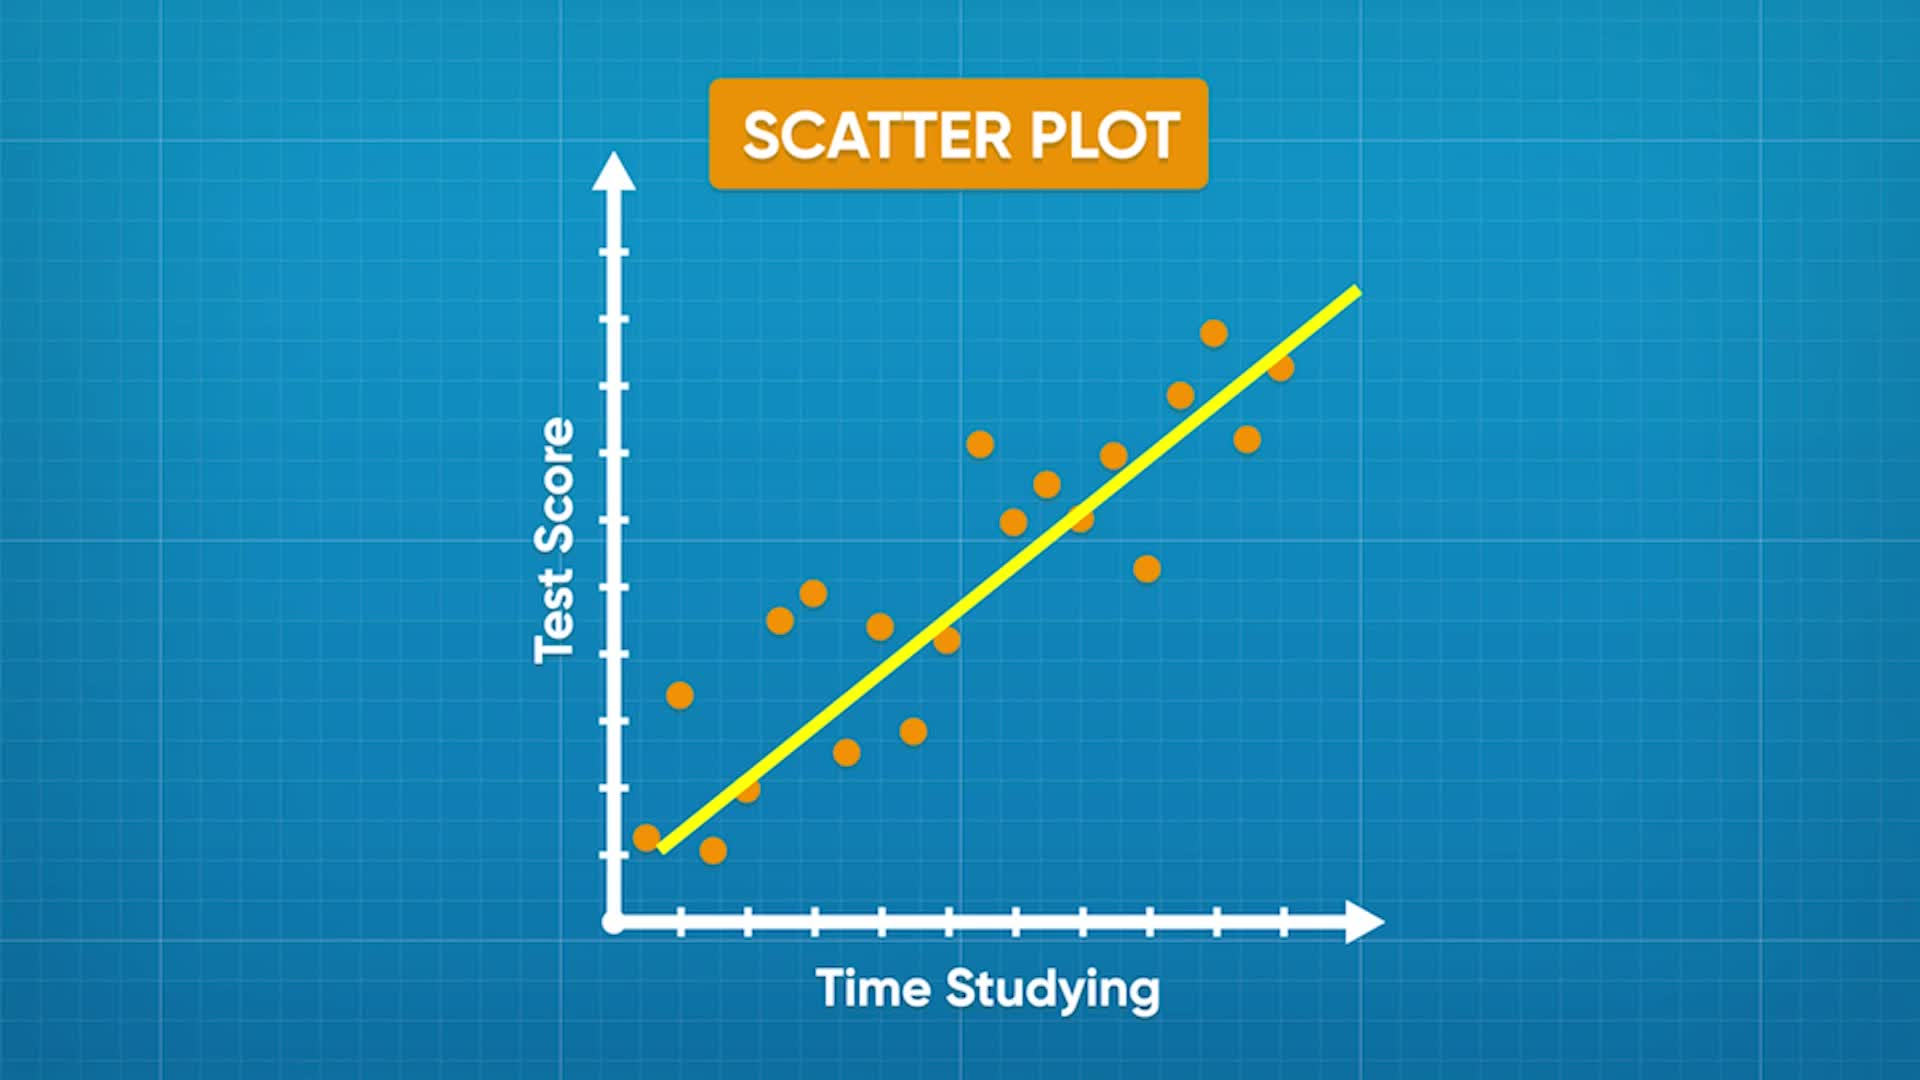
\includegraphics[width=\textwidth]{figures/bivariate.jpg}

\end{column}

\begin{column}{0.42\textwidth}

The figure represents bivariate data by showing the
relationship between two variables.

\vspace{0.3cm}

Each point represents one observation with a value for
both variables.

\vspace{0.3cm}

\textbf{Key Observation}

The pattern of the points helps us identify whether the
two variables have a possible relationship.

\end{column}

\end{columns}

\end{frame}

% ---------------------------------------------------------
% MULTIVARIATE
% ---------------------------------------------------------

\begin{frame}{6.3 Multivariate Data}

\textbf{Definition}

Multivariate data contains observations involving three or more
variables.

\textbf{Example} A student dataset may contain:
\[
\{\text{Age, Attendance, Study Hours, Marks}\}
\]
Each observation can be represented as
\[
\mathbf{x}_i =
(x_{i1},x_{i2},\ldots,x_{ip})
\]
where $p$ is the number of variables.

\textbf{Common analysis}

\begin{itemize}
    \item Covariance matrix
    \item Correlation analysis
    \item Multiple regression
\end{itemize}

\textbf{Application:} Most real-world AI and machine learning
datasets are multivariate.

\end{frame}

% ---------------------------------------------------------
% 6.3 MULTIVARIATE DATA -- FIGURE
% ---------------------------------------------------------

\begin{frame}{6.3 Multivariate Data -- Figure}

\begin{columns}[T]

\begin{column}{0.58\textwidth}

\centering
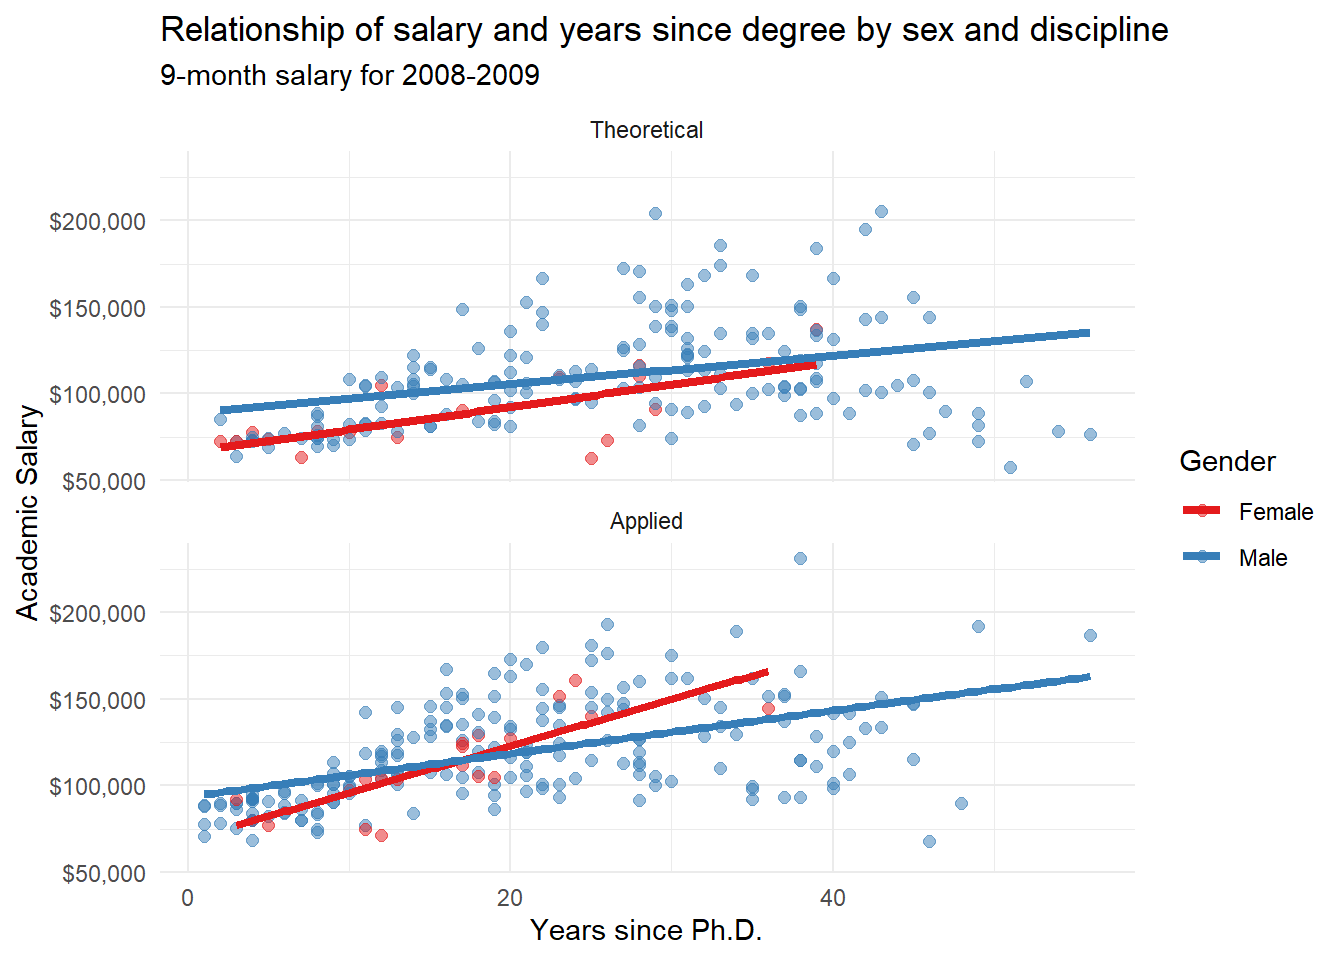
\includegraphics[width=\textwidth]{figures/multivariate.png}

\end{column}

\begin{column}{0.38\textwidth}

The figure represents data involving more than
two variables simultaneously. Each observation
contains multiple measurements.

\vspace{0.4cm}

\textbf{Observation}

The figure shows how several variables can be
examined together to identify patterns and
relationships in the data.

\end{column}

\end{columns}

\end{frame}
% =========================================================
% PART II -- DESCRIPTIVE STATISTICS
% =========================================================

\section{Descriptive Statistics}

% ---------------------------------------------------------
% 7. MEASURES OF CENTRAL TENDENCY
% ---------------------------------------------------------

\begin{frame}{7. Measures of Central Tendency}

\textbf{Definition}

Measures of central tendency describe the \textbf{central or typical
value} of a dataset.

\vspace{0.4cm}

The three commonly used measures are:

\begin{itemize}
    \item \textbf{Mean} -- arithmetic average of the observations.
    \item \textbf{Median} -- middle value after arranging the data.
    \item \textbf{Mode} -- most frequently occurring value.
\end{itemize}

\vspace{0.4cm}

\textbf{Purpose}

They provide a single value that represents the center of a dataset.

\vspace{0.3cm}

\textbf{Application:}

Used to summarize datasets in statistics, data analysis,
and machine learning.

\end{frame}


% ---------------------------------------------------------
% 7.1 MEAN -- DEFINITION AND FORMULA
% ---------------------------------------------------------

\begin{frame}{7.1 Mean}

\textbf{Definition}

The arithmetic mean is obtained by dividing the sum of all
observations by the number of observations.

\textbf{Formula}

For observations $x_1,x_2,\ldots,x_n$,
\[
\boxed{
\bar{x} = \frac{1}{n}\sum_{i=1}^{n}x_i
}
\]

where $n$ is the number of observations.

\textbf{Interpretation}

The mean represents the value obtained when the total of all
observations is distributed equally among the $n$ observations.

\textbf{Note:} The mean uses every observation in the dataset and
is therefore sensitive to extreme values.

\end{frame}


% ---------------------------------------------------------
% 7.1 MEAN -- EXAMPLE
% ---------------------------------------------------------

\begin{frame}{7.1 Mean -- Example}

\textbf{Example}

Consider the dataset:
\[
X=\{10,20,30,40,50\}
\]

There are $n=5$ observations.

\textbf{Calculation}
\[
\bar{x}
=
\frac{10+20+30+40+50}{5}
\]
\[
\boxed{\bar{x}=30}
\]

\textbf{Interpretation}

The average value of the dataset is $30$.

\textbf{Application}

The mean is widely used to summarize numerical features such as
marks, income, temperature, and sensor measurements.

\end{frame}


% ---------------------------------------------------------
% 7.2 MEDIAN -- DEFINITION AND FORMULA
% ---------------------------------------------------------

\begin{frame}{7.2 Median}

\textbf{Definition}

The median is the \textbf{middle value} of an ordered dataset.

The observations must first be arranged in ascending or
descending order.

\textbf{Formula}

For an ordered dataset with $n$ observations:
\[
\boxed{
\text{Median} =
\begin{cases}
x_{\frac{n+1}{2}}, & n \text{ is odd}\\[8pt]
\dfrac{x_{\frac{n}{2}}+x_{\frac{n}{2}+1}}{2},
& n \text{ is even}
\end{cases}
}
\]

\textbf{Key idea}

\begin{itemize}
    \item If $n$ is odd, the median is the single middle observation.
    \item If $n$ is even, the median is the average of the two middle observations.
\end{itemize}

\end{frame}


% ---------------------------------------------------------
% 7.2 MEDIAN -- EXAMPLES
% ---------------------------------------------------------

\begin{frame}{7.2 Median -- Examples}

\textbf{Example 1 -- Odd number of observations}

Consider:
\[
X=\{10,20,30,40,50\}
\]

Here, $n=5$ is odd.
\[
\text{Median}
=
x_{\frac{5+1}{2}}
=
x_3
=
\boxed{30}
\]

\vspace{0.1cm}

\textbf{Example 2 -- Even number of observations}

Consider:

\[
X=\{10,20,30,40\}
\]

Here, $n=4$ is even.

\[
\text{Median}
=
\frac{x_2+x_3}{2}
=
\frac{20+30}{2}
=
\boxed{25}
\]

\end{frame}


% ---------------------------------------------------------
% 7.3 MEDIAN -- OUTLIER EFFECT
% ---------------------------------------------------------

\begin{frame}{7.3 Median and Outliers}

\textbf{Example}

Consider:
\[
X=\{10,20,30,40,1000\}
\]

The mean is
\[
\bar{x}
=
\frac{10+20+30+40+1000}{5}
=
220
\]

while the median is
\[
\text{Median}=30
\]

\vspace{0.1cm}
\textbf{Interpretation}

The extreme value $1000$ greatly increases the mean, while the
median remains close to the center of the majority of observations.

\textbf{Key Point}

\begin{itemize}
    \item Mean is sensitive to extreme values.
    \item Median is more resistant to outliers.
\end{itemize}

\end{frame}


% ---------------------------------------------------------
% 7.4 MODE
% ---------------------------------------------------------

\begin{frame}{7.4 Mode}

\textbf{Definition}

The mode is the value that occurs with the \textbf{highest frequency}
in a dataset.

\textbf{Example}

Consider:
\[
X=\{2,4,4,5,6,4,7,8\}
\]

Therefore,
\[
\boxed{\text{Mode}=4}
\]
\textbf{Types}
\begin{itemize}
    \item \textbf{Unimodal} -- one mode.
    \item \textbf{Bimodal} -- two modes.
    \item \textbf{Multimodal} -- more than two modes.
\end{itemize}

\textbf{Application:}

Useful for identifying the most common category or value,
especially for categorical data.

\end{frame}


% ---------------------------------------------------------
% 7.5 COMPARISON
% ---------------------------------------------------------

\begin{frame}{7.5 Mean, Median and Mode}

\small

\begin{table}
\centering

\begin{tabular}{>{\bfseries}l l l}
\toprule
Measure & Main Idea & Sensitivity to Outliers \\
\midrule
Mean & Arithmetic average & High \\
Median & Middle value & Low \\
Mode & Most frequent value & Generally low \\
\bottomrule
\end{tabular}

\end{table}

\textbf{When to use?}

\begin{itemize}
    \item \textbf{Mean:} Suitable when the data is approximately
    symmetric and does not contain strong outliers.
    
    \item \textbf{Median:} Suitable for skewed data or data
    containing extreme values.
    
    \item \textbf{Mode:} Useful when the most frequent value or
    category is important.
\end{itemize}

\textbf{Application:}

Choosing an appropriate measure of central tendency helps
summarize real-world datasets effectively.

\end{frame}
% =========================================================
% PART II -- DESCRIPTIVE STATISTICS
% =========================================================

\section{Descriptive Statistics}

% ---------------------------------------------------------
% 8. MEASURES OF DISPERSION
% ---------------------------------------------------------

\begin{frame}{8. Measures of Dispersion}

\textbf{Definition}

Measures of dispersion describe the \textbf{spread or variability}
of observations around a central value.

\vspace{0.4cm}

Two datasets may have the same mean but different levels of
variability.

\vspace{0.4cm}

\textbf{Common measures}

\begin{itemize}
    \item \textbf{Range}
    \item \textbf{Variance}
    \item \textbf{Standard deviation}
    \item \textbf{Interquartile range (IQR)}
\end{itemize}

\vspace{0.3cm}

\textbf{Purpose}

They help determine how widely the observations are distributed
and how consistent the data is.

\end{frame}


% ---------------------------------------------------------
% 8.1 RANGE -- DEFINITION AND FORMULA
% ---------------------------------------------------------

\begin{frame}{8.1 Range}

\textbf{Definition}

The range is the difference between the \textbf{maximum} and
\textbf{minimum} values in a dataset.

\vspace{0.5cm}

\textbf{Formula}

\[
\boxed{
\text{Range} = x_{\max} - x_{\min}
}
\]

\vspace{0.5cm}

\textbf{Key idea}

\begin{itemize}
    \item Uses only the smallest and largest observations.
    \item Provides a simple measure of the total spread.
    \item Highly sensitive to extreme values.
\end{itemize}

\vspace{0.3cm}

\textbf{Application:}

Useful for obtaining a quick estimate of the spread of
numerical data.

\end{frame}


% ---------------------------------------------------------
% 8.1 RANGE -- EXAMPLE
% ---------------------------------------------------------

\begin{frame}{8.1 Range -- Example}

\textbf{Example}

Consider the dataset:

\[
X=\{10,20,30,40,50\}
\]

The minimum value is
\[
x_{\min}=10
\]

and the maximum value is
\[
x_{\max}=50
\]

\vspace{0.1cm}

Therefore,
\[
\text{Range}
=
50-10
=
\boxed{40}
\]

\vspace{0.1cm}

\textbf{Interpretation}

The observations span a total interval of $40$ units.

\end{frame}


% ---------------------------------------------------------
% 8.2 VARIANCE -- DEFINITION AND FORMULA
% ---------------------------------------------------------

\begin{frame}{8.2 Variance}

\textbf{Definition}

Variance measures the average squared deviation of observations
from their mean.

\vspace{0.1cm}

For a dataset $x_1,x_2,\ldots,x_n$ with mean $\bar{x}$,

\textbf{Population variance:}
\[
\boxed{
\sigma^2
=
\frac{1}{N}
\sum_{i=1}^{N}(x_i-\mu)^2
}
\]

\textbf{Sample variance:}
\[
\boxed{
s^2
=
\frac{1}{n-1}
\sum_{i=1}^{n}(x_i-\bar{x})^2
}
\]

\textbf{Key idea}

The deviations are squared so that positive and negative
deviations do not cancel each other.

\end{frame}


% ---------------------------------------------------------
% 8.2 VARIANCE -- EXAMPLE
% ---------------------------------------------------------

\begin{frame}{8.2 Variance -- Example}

\textbf{Example}

Consider:
\[
X=\{2,4,6\}
\]

First calculate the mean:
\[
\bar{x}
=
\frac{2+4+6}{3}
=
4
\]

Squared deviations:
\[
(2-4)^2=4,\qquad
(4-4)^2=0,\qquad
(6-4)^2=4
\]

Population variance:
\[
\sigma^2
=
\frac{4+0+4}{3}
=
\boxed{\frac{8}{3}}
\]

\textbf{Interpretation}

A larger variance indicates greater spread around the mean.

\end{frame}


% ---------------------------------------------------------
% 8.3 STANDARD DEVIATION -- DEFINITION AND FORMULA
% ---------------------------------------------------------

\begin{frame}{8.3 Standard Deviation}

\textbf{Definition}

Standard deviation is the positive square root of the variance.

\textbf{Population standard deviation}
\[
\boxed{
\sigma
=
\sqrt{
\frac{1}{N}
\sum_{i=1}^{N}(x_i-\mu)^2
}
}
\]
\textbf{Sample standard deviation}
\[
\boxed{
s
=
\sqrt{
\frac{1}{n-1}
\sum_{i=1}^{n}(x_i-\bar{x})^2
}
}
\]

Standard deviation is expressed in the \textbf{same units as the
original data}, unlike variance.

\end{frame}


% ---------------------------------------------------------
% 8.3 STANDARD DEVIATION -- EXAMPLE
% ---------------------------------------------------------

\begin{frame}{8.3 Standard Deviation -- Example}

\textbf{Example}

For the dataset
\[
X=\{2,4,6\},
\]
\[
\sigma^2=\frac{8}{3}
\]
Therefore,
\[
\sigma
=
\sqrt{\frac{8}{3}}
\approx
\boxed{1.63}
\]
\textbf{Interpretation}

The standard deviation indicates the typical magnitude of
deviation of observations from the mean.

\textbf{Application}

Standard deviation is widely used in data analysis and machine
learning to measure feature variability.

\end{frame}


% ---------------------------------------------------------
% 8.4 INTERQUARTILE RANGE -- DEFINITION AND FORMULA
% ---------------------------------------------------------

\begin{frame}{8.4 Interquartile Range (IQR)}

\textbf{Definition}

The interquartile range measures the spread of the
\textbf{middle 50\%} of the observations.

\vspace{0.4cm}

The data is divided into four parts using quartiles:

\begin{itemize}
    \item $Q_1$ -- First quartile (25th percentile)
    \item $Q_2$ -- Second quartile (50th percentile / median)
    \item $Q_3$ -- Third quartile (75th percentile)
\end{itemize}

\vspace{0.3cm}

\textbf{Formula}

\[
\boxed{
IQR=Q_3-Q_1
}
\]

\vspace{0.3cm}

\textbf{Key idea}

IQR focuses on the middle portion of the data and is
less affected by extreme observations.

\end{frame}


% ---------------------------------------------------------
% 8.4 IQR -- EXAMPLE
% ---------------------------------------------------------

% ---------------------------------------------------------
% 8.4 IQR -- EXAMPLE 1
% ---------------------------------------------------------

% ---------------------------------------------------------
% 8.4 IQR -- EXAMPLE 1
% ---------------------------------------------------------

\begin{frame}{8.4 Interquartile Range -- Example}

\textbf{Example}

Consider the ordered dataset:
\[
X=\{1,2,3,4,5,6,7,8,9\}
\]

The median is
\[
Q_2=5
\]

\textbf{Lower half}
\[
\{1,2,3,4\}
\]

Therefore,
\[
Q_1
=
\frac{2+3}{2}
=
\boxed{2.5}
\]

\end{frame}


% ---------------------------------------------------------
% 8.4 IQR -- EXAMPLE 2
% ---------------------------------------------------------

\begin{frame}{8.4 Interquartile Range -- Example}

\textbf{Upper half}

\[
\{6,7,8,9\}
\]

Therefore,

\[
Q_3
=
\frac{7+8}{2}
=
\boxed{7.5}
\]

From the previous example:

\[
Q_1=2.5,
\qquad
Q_3=7.5
\]

\textbf{Quartiles}

\[
Q_1=2.5,
\qquad
Q_2=5,
\qquad
Q_3=7.5
\]

\end{frame}


% ---------------------------------------------------------
% 8.4 IQR -- CALCULATION
% ---------------------------------------------------------

\begin{frame}{8.4 Interquartile Range -- Calculation}

\textbf{Formula}
\[
\boxed{IQR=Q_3-Q_1}
\]

\textbf{Calculation}

Using
\[
Q_1=2.5,
\qquad
Q_3=7.5
\]
we get
\[
IQR=7.5-2.5
\]
\[
\boxed{IQR=5}
\]

\textbf{Interpretation}

The interquartile range is $5$, meaning that the middle
$50\%$ of the observations are spread over an interval of
$5$ units.

\textbf{Key Point}

IQR is less affected by extreme values than the range.

\end{frame}

% ---------------------------------------------------------
% 8.5 COMPARISON OF DISPERSION MEASURES
% ---------------------------------------------------------

\begin{frame}{8.5 Comparison of Dispersion Measures}

\small

\begin{table}
\centering

\begin{tabular}{>{\bfseries}l l l}
\toprule
Measure & What it describes & Outlier sensitivity \\
\midrule
Range & Total spread & High \\
Variance & Squared deviation from mean & High \\
Standard deviation & Spread around mean & High \\
IQR & Spread of middle 50\% & Low \\
\bottomrule
\end{tabular}

\end{table}

\vspace{0.4cm}

\textbf{When to use?}

\begin{itemize}
    \item \textbf{Range:} Quick measure of total spread.
    \item \textbf{Variance:} Useful in statistical and mathematical models.
    \item \textbf{Standard deviation:} Easy to interpret in the original units.
    \item \textbf{IQR:} Useful for skewed data and datasets with outliers.
\end{itemize}

\end{frame}
% =========================================================
% PART II -- DESCRIPTIVE STATISTICS
% =========================================================

\section{Descriptive Statistics}

% ---------------------------------------------------------
% 9. HISTOGRAM
% ---------------------------------------------------------

\begin{frame}{9. Histogram}

\textbf{Definition}

A histogram is a graphical representation of the distribution
of numerical data using \textbf{continuous intervals called bins}.

\vspace{0.1cm}

\textbf{Key features}

\begin{itemize}
    \item The horizontal axis represents the range of values.
    \item The vertical axis represents frequency or count.
    \item Adjacent bars touch because the intervals are continuous.
\end{itemize}

\vspace{0.1cm}

\textbf{Purpose}

A histogram helps identify the shape, center, spread, and
possible unusual patterns in a dataset.

\vspace{0.1cm}

\textbf{Application}

Histograms are commonly used in exploratory data analysis
to understand the distribution of numerical features.

\end{frame}

% ---------------------------------------------------------
% 9.1 HISTOGRAM -- FIGURE
% ---------------------------------------------------------

\begin{frame}{9.1 Histogram -- Figure}

\begin{columns}[T]

\begin{column}{0.62\textwidth}

\centering
\includegraphics[width=\textwidth]{figures/histogram.png}

\end{column}

\begin{column}{0.34\textwidth}

The observations are grouped into intervals
called bins. The height of each bar represents
the frequency of observations in that interval.

\vspace{0.4cm}

\textbf{Observation}

The overall shape of the bars provides a visual
indication of the distribution of the data.

\end{column}

\end{columns}

\end{frame}

% ---------------------------------------------------------
% 9.2 HISTOGRAM -- EXAMPLE
% ---------------------------------------------------------

\begin{frame}{9.2 Histogram -- Example}

\textbf{Example}

Consider the marks of students:
\[
X=\{42,45,48,51,52,55,57,58,61,63,
65,66,68,70,72\}
\]

The observations can be grouped into intervals such as:
\[
\begin{array}{c|c}
\text{Marks Interval} & \text{Frequency}\\
\hline
40-49 & 3\\
50-59 & 5\\
60-69 & 4\\
70-79 & 3
\end{array}
\]

The histogram represents these frequencies using adjacent
bars for the intervals.

\textbf{Interpretation}

The distribution can be examined to understand where the
observations are concentrated.

\end{frame}


% ---------------------------------------------------------
% 9.3 HISTOGRAM -- INTERPRETATION
% ---------------------------------------------------------

\begin{frame}{9.3 Histogram -- Interpretation}

A histogram can reveal important characteristics of a dataset.

\vspace{0.3cm}

\begin{itemize}
    \item \textbf{Center:} Where most observations are concentrated.
    
    \item \textbf{Spread:} How widely the observations are distributed.
    
    \item \textbf{Shape:} Whether the distribution is symmetric,
    skewed, or has multiple peaks.
    
    \item \textbf{Possible outliers:} Observations that appear
    far from the main concentration.
\end{itemize}

\vspace{0.4cm}

\textbf{Application in AI}

Histograms can be used during exploratory data analysis to
understand feature distributions before preprocessing or
model building.

\end{frame}


% ---------------------------------------------------------
% 10. BOX PLOT
% ---------------------------------------------------------

\begin{frame}{10. Box Plot}

\textbf{Definition}

A box plot is a graphical representation of a dataset based on
its \textbf{five-number summary}.

\vspace{0.1cm}

\textbf{Five-number summary}

\begin{itemize}
    \item Minimum
    \item First quartile ($Q_1$)
    \item Median ($Q_2$)
    \item Third quartile ($Q_3$)
    \item Maximum
\end{itemize}

The box represents the interval from $Q_1$ to $Q_3$.
\[
\boxed{IQR=Q_3-Q_1}
\]

\vspace{0.1cm}

\textbf{Purpose}

A box plot summarizes the center, spread and potential
outliers of numerical data.

\end{frame}


% ---------------------------------------------------------
% 10.1 BOX PLOT -- COMPONENTS
% ---------------------------------------------------------

\begin{frame}{10.1 Box Plot -- Components}

\textbf{Main components}

\begin{itemize}
    \item \textbf{Lower whisker} -- lower end of the non-outlier range.
    \item \textbf{Box} -- extends from $Q_1$ to $Q_3$.
    \item \textbf{Median line} -- represents $Q_2$.
    \item \textbf{Upper whisker} -- upper end of the non-outlier range.
    \item \textbf{Points beyond whiskers} -- potential outliers.
\end{itemize}

\vspace{0.1cm}

\textbf{Outlier rule}

An observation is commonly considered an outlier if
\[
x<Q_1-1.5(IQR)
\]

or
\[
x>Q_3+1.5(IQR)
\]

The box plot provides a compact summary of the distribution
and is particularly useful for comparing multiple datasets.

\end{frame}

% ---------------------------------------------------------
% 10.2 BOX PLOT -- FIGURE
% ---------------------------------------------------------

\begin{frame}{10.2 Box Plot -- Figure}

\begin{columns}[c]

\begin{column}{0.43\textwidth}

\centering
\includegraphics[width=\textwidth]{figures/boxplot.png}

\end{column}

\begin{column}{0.42\textwidth}

\vspace{0.2cm}

The box represents the middle $50\%$ of the
data, from $Q_1$ to $Q_3$. The line inside the
box represents the median.

\vspace{0.3cm}

The whiskers extend toward the lower and upper
values that are not considered potential outliers.

\end{column}

\end{columns}

\end{frame}

% ---------------------------------------------------------
% 10.3 BOX PLOT -- EXAMPLE
% ---------------------------------------------------------

\begin{frame}{10.3 Box Plot -- Example}

\textbf{Example}

Consider the ordered dataset:
\[
X=\{1,2,3,4,5,6,7,8,9\}
\]

The quartiles are:
\[
Q_1=2.5,\qquad Q_2=5,\qquad Q_3=7.5
\]

Therefore,
\[
IQR=Q_3-Q_1
=
7.5-2.5
=
5
\]

\vspace{0.1cm}

The lower and upper outlier boundaries are:
\[
Q_1-1.5(IQR)
=
2.5-7.5
=
-5
\]
\[
Q_3+1.5(IQR)
=
7.5+7.5
=
15
\]

Since all observations lie between $-5$ and $15$,
there are no outliers.

\end{frame}


% ---------------------------------------------------------
% 11. OUTLIERS
% ---------------------------------------------------------

\begin{frame}{11. Outliers}

\textbf{Definition}

An outlier is an observation that lies unusually far from
the general pattern of the dataset.

\textbf{Common causes}

\begin{itemize}
    \item Measurement or data-entry errors
    \item Unusual events
    \item Natural variation
    \item Rare observations
\end{itemize}

\textbf{Effect}

Outliers can strongly influence statistical measures such as
the mean, variance, and standard deviation.

\textbf{Important}

An outlier is not necessarily an error. It should be investigated
before deciding whether to remove or transform it.

\end{frame}

% ---------------------------------------------------------
% 11.1 OUTLIERS -- FIGURE
% ---------------------------------------------------------

\begin{frame}{11.1 Outliers -- Figure}

\begin{columns}[c]

\begin{column}{0.62\textwidth}

\centering
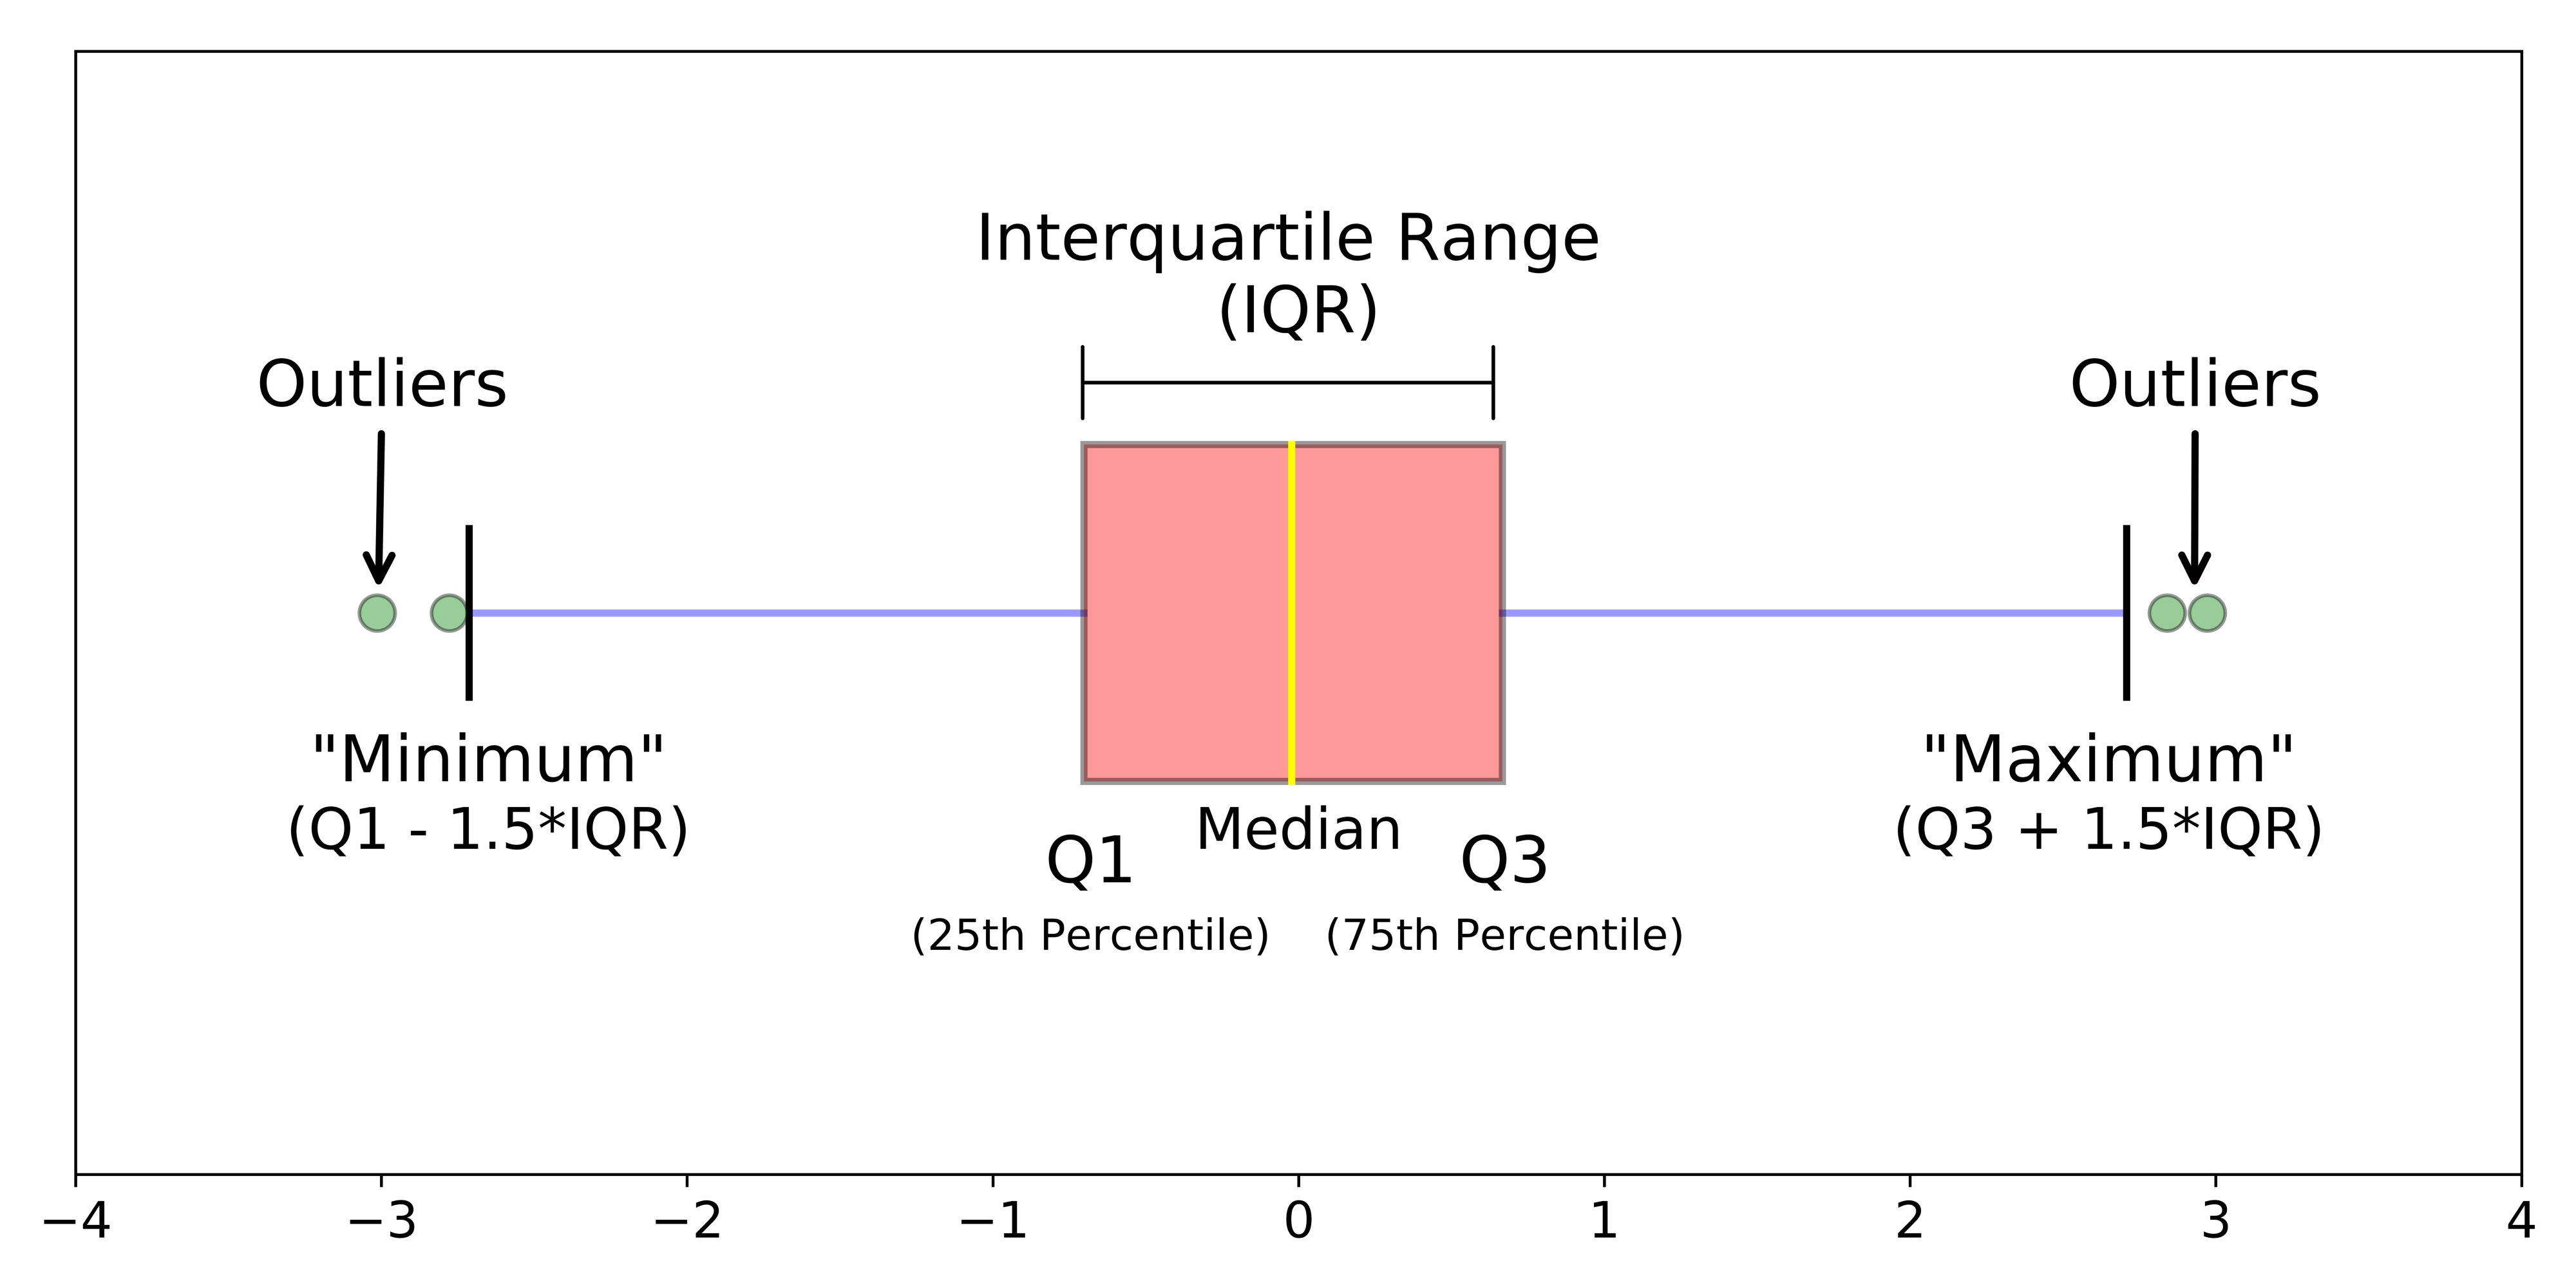
\includegraphics[width=\textwidth]{figures/outlier.png}

\end{column}

\begin{column}{0.34\textwidth}

\vspace{0.2cm}

The figure shows an observation located far
from the main group of observations.

\vspace{0.2cm}

Such observations may strongly influence
statistics such as the mean and variance.

\end{column}

\end{columns}

\end{frame}


% ---------------------------------------------------------
% 11.2 OUTLIERS -- IQR METHOD
% ---------------------------------------------------------

\begin{frame}{11.2 Outliers -- IQR Method}

The IQR method identifies potential outliers using the
first and third quartiles.

\textbf{Step 1: Calculate IQR}
\[
IQR=Q_3-Q_1
\]

\textbf{Step 2: Calculate the boundaries}
\[
\boxed{
\text{Lower Bound}=Q_1-1.5(IQR)
}
\]
\[
\boxed{
\text{Upper Bound}=Q_3+1.5(IQR)
}
\]

\textbf{Step 3: Identify potential outliers}
\[
x<\text{Lower Bound}
\]
or
\[
x>\text{Upper Bound}
\]
Observations outside these boundaries are treated as
potential outliers.

\end{frame}


% ---------------------------------------------------------
% 12. SKEWNESS
% ---------------------------------------------------------

\begin{frame}{12. Skewness}

\textbf{Definition}

Skewness measures the \textbf{asymmetry} of a probability
distribution or dataset around its mean.

\vspace{0.1cm}

\textbf{Types}

\begin{itemize}
    \item \textbf{Symmetric:} Distribution is approximately balanced.
    
    \item \textbf{Right-skewed:} Longer tail extends toward larger values.
    
    \item \textbf{Left-skewed:} Longer tail extends toward smaller values.
\end{itemize}

\vspace{0.1cm}

\textbf{Interpretation}
\[
\text{Right skewness} \Rightarrow
\text{Mean}>\text{Median}
\]
\[
\text{Left skewness} \Rightarrow
\text{Mean}<\text{Median}
\]

\textbf{Application}

Skewness is useful when deciding whether mean or median
is a more appropriate measure of central tendency.

\end{frame}

% ---------------------------------------------------------
% 12.1 SKEWNESS -- FIGURE
% ---------------------------------------------------------

\begin{frame}{12.1 Skewness -- Figure}

\begin{columns}[T]

\begin{column}{0.50\textwidth}

\centering
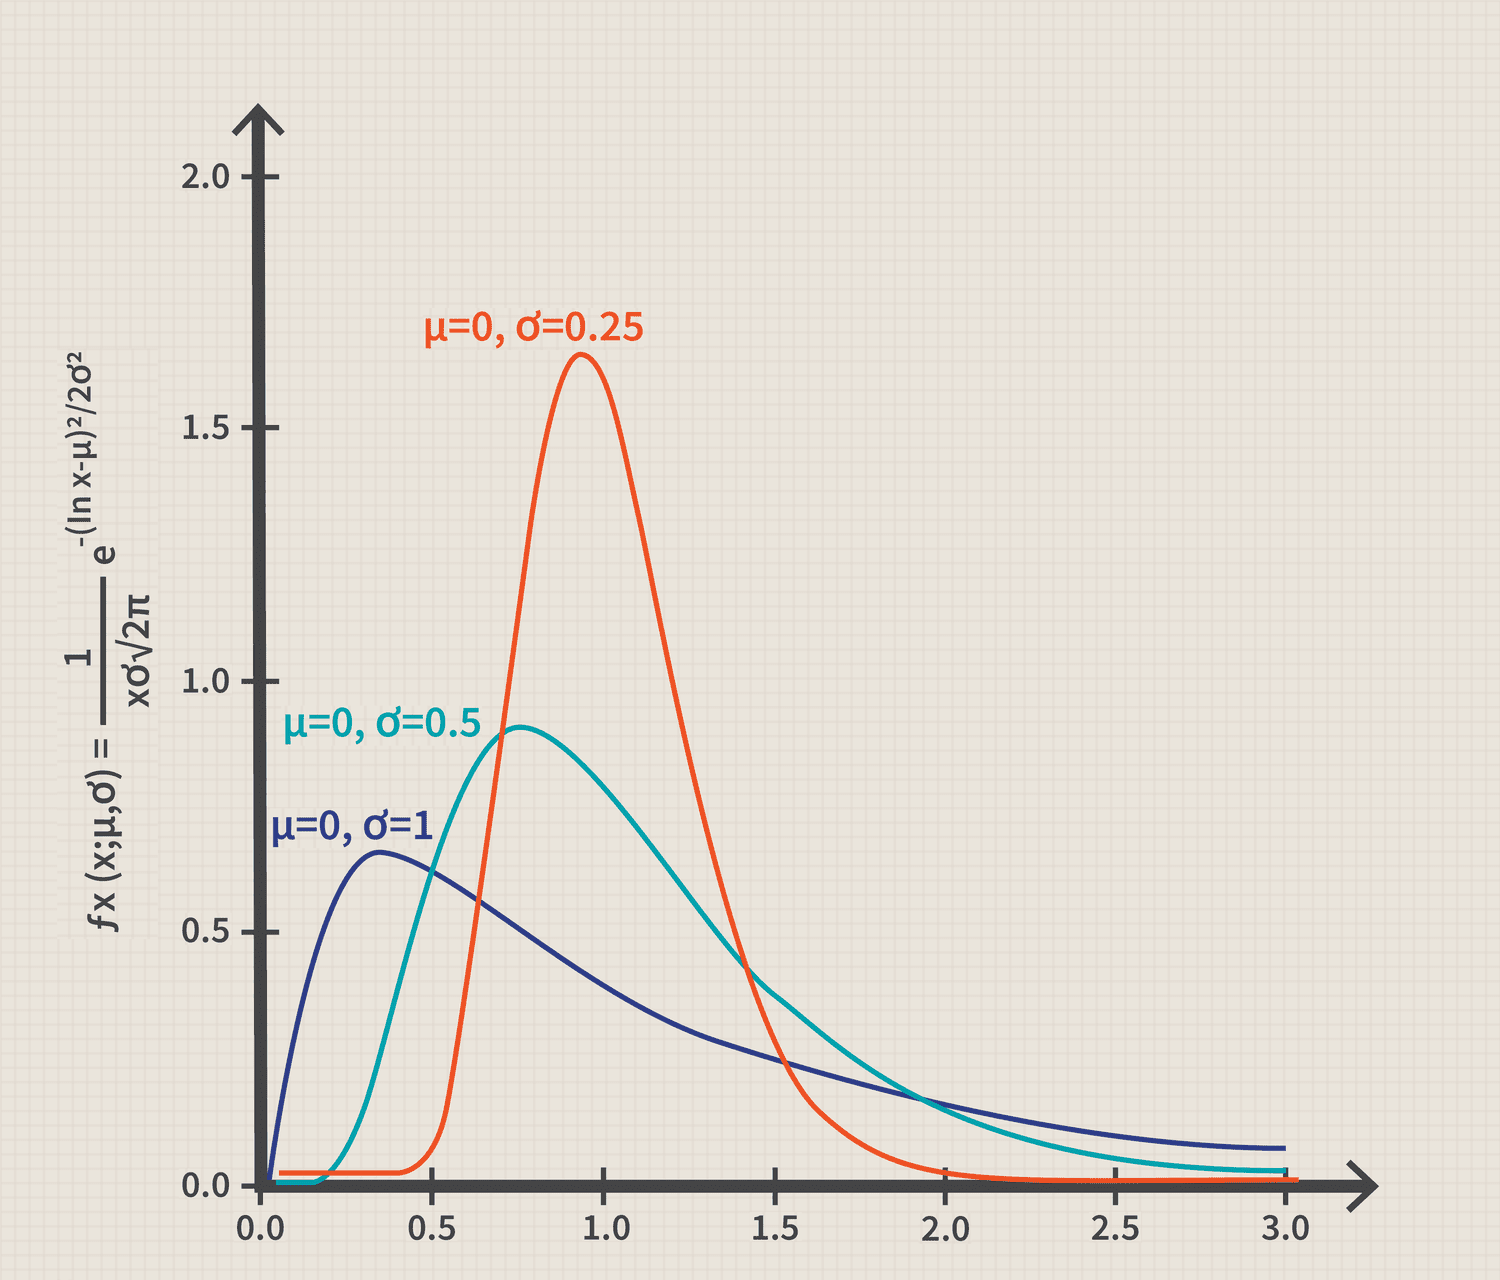
\includegraphics[width=\textwidth]{figures/skewness.png}

\end{column}

\begin{column}{0.34\textwidth}

The figure compares distributions with
different directions of asymmetry.

\vspace{0.3cm}

A longer tail toward the left indicates
negative skewness, while a longer tail toward
the right indicates positive skewness.

\vspace{0.3cm}

A symmetric distribution has approximately
equal tails on both sides.

\end{column}

\end{columns}

\end{frame}

% ---------------------------------------------------------
% 12.2 SKEWNESS -- EXAMPLE
% ---------------------------------------------------------

\begin{frame}{12.2 Skewness -- Example}

\textbf{Example: Income Distribution}

Suppose most people in a dataset have moderate incomes,
while a small number have very high incomes.

\vspace{0.1cm}

The distribution will have a long tail toward larger values.

\[
\boxed{\text{Right-skewed distribution}}
\]

\vspace{0.1cm}

Typically,

\[
\text{Mean}>\text{Median}
\]

because the few high-income observations pull the mean
toward the right.

\end{frame}

% ---------------------------------------------------------
% 12.3 SKEWNESS -- APPLICATION
% ---------------------------------------------------------

\begin{frame}{12.3 Skewness -- Application}

\textbf{Application}

Income, house prices, transaction amounts, and many financial
variables can exhibit right-skewed distributions.

\vspace{0.3cm}

\textbf{Why it matters in AI}

Highly skewed features can affect statistical analysis and
machine learning models.

\vspace{0.3cm}

Possible preprocessing techniques include:

\begin{itemize}
    \item Log transformation
    \item Robust scaling
    \item Other suitable transformations
\end{itemize}

\end{frame}

% ---------------------------------------------------------
% 13. KURTOSIS
% ---------------------------------------------------------

\begin{frame}{13. Kurtosis}

\textbf{Definition}

Kurtosis describes the degree to which a distribution has
\textbf{heavy or light tails} relative to a normal distribution.

\vspace{0.4cm}

It is related to the tendency of a distribution to produce
extreme observations.

\vspace{0.3cm}

\textbf{Types}

\begin{itemize}
    \item \textbf{Mesokurtic:} Similar tail behaviour to a normal distribution.
    
    \item \textbf{Leptokurtic:} Heavier tails and greater tendency
    for extreme observations.
    
    \item \textbf{Platykurtic:} Lighter tails and fewer extreme observations.
\end{itemize}

\vspace{0.3cm}

\textbf{Application}

Kurtosis is useful when analyzing distributions where the
presence of extreme observations is important.

\end{frame}


% ---------------------------------------------------------
% 13.1 KURTOSIS -- EXCESS KURTOSIS
% ---------------------------------------------------------

\begin{frame}{13.1 Kurtosis -- Excess Kurtosis}

For a random variable $X$ with mean $\mu$ and standard deviation
$\sigma$, kurtosis can be expressed as
\[
\boxed{
K=
\frac{E[(X-\mu)^4]}{\sigma^4}
}
\]

The \textbf{excess kurtosis} is
\[
\boxed{
K_{\text{excess}}=K-3
}
\]

For a normal distribution:
\[
K=3
\]

and therefore
\[
K_{\text{excess}}=0
\]

\vspace{0.1cm}

\textbf{Interpretation}

Higher kurtosis generally indicates heavier tails and a
greater tendency for extreme observations.

\end{frame}

% ---------------------------------------------------------
% 13.2 KURTOSIS -- FIGURE
% ---------------------------------------------------------

\begin{frame}{13.2 Kurtosis -- Figure}

\begin{columns}[T]

\begin{column}{0.62\textwidth}

\centering
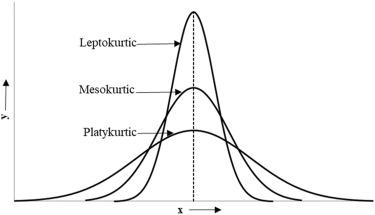
\includegraphics[width=\textwidth]{figures/kurtosis.jpg}

\end{column}

\begin{column}{0.34\textwidth}


The figure compares distributions with
different tail behaviors.

\vspace{0.4cm}

Distributions with heavier tails have a greater
tendency to produce observations far from the
center.

\end{column}

\end{columns}

\end{frame}

% ---------------------------------------------------------
% 13.3 SKEWNESS VS KURTOSIS
% ---------------------------------------------------------

\begin{frame}{13.3 Skewness vs Kurtosis}

\small

\begin{table}
\centering

\begin{tabular}{>{\bfseries}l l}
\toprule
Measure & Describes \\
\midrule
Skewness & Asymmetry of the distribution \\
Kurtosis & Tail heaviness / tendency toward extremes \\
\bottomrule
\end{tabular}

\end{table}

\vspace{0.5cm}

\textbf{Key distinction}

\begin{itemize}
    \item \textbf{Skewness} focuses on the direction and degree
    of asymmetry.
    
    \item \textbf{Kurtosis} focuses mainly on the behaviour of
    the tails and extreme observations.
\end{itemize}

\vspace{0.3cm}

\textbf{Application in AI}

Both measures can help identify unusual feature distributions
and guide data preprocessing and exploratory analysis.

\end{frame}
% =========================================================
% PART III -- SAMPLE STATISTICS
% =========================================================

\section{Sample Statistics}

% ---------------------------------------------------------
% 14. POPULATION AND SAMPLE
% ---------------------------------------------------------

\begin{frame}{14. Population and Sample}

\textbf{Population}

A population is the \textbf{complete set of individuals,
objects, or observations} of interest in a study.

\vspace{0.4cm}

\textbf{Sample}

A sample is a \textbf{subset of the population} selected for
analysis.

\vspace{0.4cm}

\[
\boxed{
\text{Population}
\supseteq
\text{Sample}
}
\]

\vspace{0.3cm}

\textbf{Example}

If a university has 5,000 students and we select 200 students
for analysis:

\begin{itemize}
    \item Population = 5,000 students
    \item Sample = 200 selected students
\end{itemize}

\end{frame}

% ---------------------------------------------------------
% 14.1 POPULATION AND SAMPLE -- FIGURE
% ---------------------------------------------------------

\begin{frame}{14.1 Population and Sample -- Figure}

\begin{columns}[T]

\begin{column}{0.55\textwidth}

\centering
\includegraphics[width=\textwidth]{figures/population_sample.png}

\end{column}

\begin{column}{0.46\textwidth}

The figure illustrates the relationship between a population, a sampling frame, and a sample in a research study.

\vspace{0.1cm}

The large gray circle represents the population, the entire target population under study.

\vspace{0.1cm}

The blue circle inside it represents the sampling frame, the portion of the target population from which participants can be selected.

\vspace{0.1cm}

The dark navy circle represents the sample, the actual units or individuals selected for the study.

\end{column}

\end{columns}

\end{frame}

% ---------------------------------------------------------
% 14.2 POPULATION VS SAMPLE
% ---------------------------------------------------------

\begin{frame}{14.2 Population and Sample -- Comparison}

\small

\begin{table}
\centering

\begin{tabular}{>{\bfseries}l l l}
\toprule
 & Population & Sample \\
\midrule
Size & Complete set & Subset \\
Mean & $\mu$ & $\bar{x}$ \\
Variance & $\sigma^2$ & $s^2$ \\
Standard deviation & $\sigma$ & $s$ \\
Purpose & Describe population & Estimate population \\
\bottomrule
\end{tabular}

\end{table}

\vspace{0.5cm}

\textbf{Key idea}

Since studying an entire population may be expensive or
impractical, statistical analysis often uses a sample to
learn about the population.

\vspace{0.3cm}

\textbf{Application}

Sampling is fundamental in machine learning, surveys,
experiments and data analysis.

\end{frame}


% ---------------------------------------------------------
% 15. SAMPLE MEAN
% ---------------------------------------------------------

\begin{frame}{15. Sample Mean}

\textbf{Definition}

The sample mean is the arithmetic average of the observations
in a sample.

For a sample
\[
x_1,x_2,\ldots,x_n
\]

the sample mean is
\[
\boxed{
\bar{x}
=
\frac{1}{n}
\sum_{i=1}^{n}x_i
}
\]

\vspace{0.1cm}

\textbf{Interpretation}

The sample mean provides an estimate of the population mean $\mu$.

\[
\boxed{
\bar{x}\approx\mu
}
\]

The quality of this estimate generally improves as the sample
size increases.

\end{frame}


% ---------------------------------------------------------
% 15.1 SAMPLE MEAN -- EXAMPLE
% ---------------------------------------------------------

\begin{frame}{15.1 Sample Mean -- Example}

\textbf{Example}

Consider a sample of five observations:

\[
X=\{12,15,18,20,25\}
\]

The sample mean is

\[
\bar{x}
=
\frac{12+15+18+20+25}{5}
\]

\[
\boxed{
\bar{x}=18
}
\]

\vspace{0.4cm}

\textbf{Interpretation}

The value $18$ is the average of the observations in the
sample and can be used as an estimate of the population mean.

\end{frame}


% ---------------------------------------------------------
% 16. SAMPLE VARIANCE
% ---------------------------------------------------------

\begin{frame}{16. Sample Variance}

\textbf{Definition}

Sample variance measures the variability of observations
around the sample mean.

\vspace{0.4cm}

For a sample $x_1,x_2,\ldots,x_n$:

\[
\boxed{
s^2
=
\frac{1}{n-1}
\sum_{i=1}^{n}
(x_i-\bar{x})^2
}
\]

\vspace{0.4cm}

\textbf{Why $n-1$?}

The denominator $n-1$ provides an unbiased estimator of the
population variance under the usual random-sampling assumptions.

\vspace{0.3cm}

\textbf{Key idea}

Sample variance measures how much the observations vary
around their sample mean.

\end{frame}


% ---------------------------------------------------------
% 16.1 SAMPLE VARIANCE -- EXAMPLE
% ---------------------------------------------------------

\begin{frame}{16.1 Sample Variance -- Example}

\textbf{Example}

Consider:
\[
X=\{2,4,6\}
\]
The sample mean is
\[
\bar{x}=4
\]
Squared deviations:
\[
(2-4)^2=4,\qquad
(4-4)^2=0,\qquad
(6-4)^2=4
\]
\[
s^2
=
\frac{4+0+4}{3-1}
\]
\[
\boxed{s^2=4}
\]
\textbf{Interpretation}

The sample variance quantifies the spread of the observations
around their sample mean.

\end{frame}


% ---------------------------------------------------------
% 17. ORDER STATISTICS
% ---------------------------------------------------------

\begin{frame}{17. Order Statistics}

\textbf{Definition}

Order statistics are the observations arranged in
\textbf{ascending order}.

\vspace{0.1cm}

Given observations
\[
x_1,x_2,\ldots,x_n,
\]

their ordered values are written as
\[
\boxed{
x_{(1)}\leq x_{(2)}\leq\cdots\leq x_{(n)}
}
\]

where $x_{(i)}$ denotes the $i$-th smallest observation.

\vspace{0.1cm}

\textbf{Examples of order statistics}

\begin{itemize}
    \item $x_{(1)}$ -- minimum
    \item $x_{(n)}$ -- maximum
    \item Middle order statistic -- median
    \item Quartiles -- divide ordered data into parts
\end{itemize}

\end{frame}


% ---------------------------------------------------------
% 17.1 ORDER STATISTICS -- EXAMPLE
% ---------------------------------------------------------

\begin{frame}{17.1 Order Statistics -- Example}

\textbf{Example}

Consider:
\[
X=\{40,10,30,50,20\}
\]

Arrange the observations in ascending order:
\[
10,\;20,\;30,\;40,\;50
\]
Therefore,
\[
x_{(1)}=10,\qquad
x_{(2)}=20,\qquad
x_{(3)}=30,\qquad
x_{(4)}=40,\qquad
x_{(5)}=50
\]
Hence,
\[
\boxed{x_{(1)}=\min(X)}
\]
\[
\boxed{x_{(5)}=\max(X)}
\]

The middle observation $x_{(3)}=30$ is the median.

\end{frame}


% ---------------------------------------------------------
% 18. COVARIANCE
% ---------------------------------------------------------

\begin{frame}{18. Covariance}

\textbf{Definition}

Covariance measures the \textbf{direction of the linear
relationship} between two variables.

\vspace{0.4cm}

For random variables $X$ and $Y$:

\[
\boxed{
\operatorname{Cov}(X,Y)
=
E[(X-\mu_X)(Y-\mu_Y)]
}
\]

\vspace{0.4cm}

\textbf{Interpretation}

\begin{itemize}
    \item Positive covariance: variables tend to increase together.
    \item Negative covariance: one tends to increase when the other decreases.
    \item Covariance near zero: weak linear association.
\end{itemize}

\vspace{0.3cm}

\textbf{Note}

The magnitude of covariance depends on the units of the variables.

\end{frame}


% ---------------------------------------------------------
% 18.1 COVARIANCE -- EXAMPLE
% ---------------------------------------------------------

\begin{frame}{18.1 Covariance -- Example}

\textbf{Example}

Consider two variables:
\[
X=\{1,2,3\}
\]
\[
Y=\{2,4,6\}
\]
As $X$ increases, $Y$ also increases.
Their means are:
\[
\bar{x}=2,\qquad \bar{y}=4
\]
The deviations have the same sign:
\[
(-1)(-2),\quad (0)(0),\quad (1)(2)
\]
All products are non-negative.
Therefore, the covariance is \textbf{positive}.

\textbf{Interpretation}

The variables show a positive linear relationship.

\end{frame}


% ---------------------------------------------------------
% 19. SAMPLE COVARIANCE
% ---------------------------------------------------------

\begin{frame}{19. Sample Covariance}

\textbf{Definition}

Sample covariance measures the linear relationship between
two variables using sample observations.

\vspace{0.1cm}

For paired observations
\[
(x_1,y_1),(x_2,y_2),\ldots,(x_n,y_n),
\]

the sample covariance is
\[
\boxed{
s_{XY}
=
\frac{1}{n-1}
\sum_{i=1}^{n}
(x_i-\bar{x})(y_i-\bar{y})
}
\]

\vspace{0.1cm}

\textbf{Interpretation}

\begin{itemize}
    \item $s_{XY}>0$: positive association.
    \item $s_{XY}<0$: negative association.
    \item $s_{XY}\approx0$: weak linear association.
\end{itemize}

\end{frame}

% ---------------------------------------------------------
% 19.1 SAMPLE COVARIANCE -- EXAMPLE
% ---------------------------------------------------------

\begin{frame}{19.1 Sample Covariance -- Example}

\textbf{Example}

Consider two variables:
\[
X=\{1,2,3\},
\qquad
Y=\{2,4,6\}
\]

The sample means are:
\[
\bar{x}=2,
\qquad
\bar{y}=4
\]

\begin{table}
\centering
\small

\begin{tabular}{c c c c c}
\toprule
$x_i$ & $y_i$ & $x_i-\bar{x}$ & $y_i-\bar{y}$ &
Product \\
\midrule
1 & 2 & $-1$ & $-2$ & $2$ \\
2 & 4 & $0$ & $0$ & $0$ \\
3 & 6 & $1$ & $2$ & $2$ \\
\bottomrule
\end{tabular}

\end{table}
\[
s_{XY}
=
\frac{2+0+2}{3-1}
=
\boxed{2}
\]

Since $s_{XY}>0$, $X$ and $Y$ have a positive covariance
and tend to increase together.

\end{frame}

% ---------------------------------------------------------
% 20. CORRELATION
% ---------------------------------------------------------

\begin{frame}{20. Correlation}

\textbf{Definition}

Correlation is a standardized measure of the
\textbf{strength and direction of linear association}
between two variables.

\vspace{0.1cm}

The population correlation coefficient is
\[
\boxed{
\rho_{XY}
=
\frac{\operatorname{Cov}(X,Y)}
{\sigma_X\sigma_Y}
}
\]

For a sample, the corresponding measure is the
\textbf{sample correlation coefficient} $r$.
\[
\boxed{
-1\leq r\leq1
}
\]

\textbf{Interpretation}

\begin{itemize}
    \item $r=1$: perfect positive linear relationship.
    \item $r=-1$: perfect negative linear relationship.
    \item $r\approx0$: weak or no linear relationship.
\end{itemize}

\end{frame}


% ---------------------------------------------------------
% 20.1 CORRELATION -- COVARIANCE
% ---------------------------------------------------------

\begin{frame}{20.1 Correlation -- Relation to Covariance}

The sample correlation coefficient can be written as
\[
\boxed{
r
=
\frac{s_{XY}}{s_Xs_Y}
}
\]
where:

\begin{itemize}
    \item $s_{XY}$ = sample covariance
    \item $s_X$ = sample standard deviation of $X$
    \item $s_Y$ = sample standard deviation of $Y$
\end{itemize}

\vspace{0.2cm}

\textbf{Key difference}

\begin{itemize}
    \item Covariance depends on the units of measurement.
    \item Correlation is standardized and always lies between $-1$ and $1$.
\end{itemize}

\vspace{0.1cm}

\textbf{Application}

Correlation is commonly used for feature analysis and
understanding relationships between variables in datasets.

\end{frame}


% ---------------------------------------------------------
% 21. SAMPLE COVARIANCE MATRIX
% ---------------------------------------------------------

\begin{frame}{21. Sample Covariance Matrix}

\textbf{Definition}

For a dataset containing multiple variables, the sample
covariance matrix summarizes the covariance between every
pair of variables.

For $p$ variables:
\[
\boxed{
S=
\begin{bmatrix}
s_{11} & s_{12} & \cdots & s_{1p}\\
s_{21} & s_{22} & \cdots & s_{2p}\\
\vdots & \vdots & \ddots & \vdots\\
s_{p1} & s_{p2} & \cdots & s_{pp}
\end{bmatrix}
}
\]

where
\[
s_{ij}
=
\frac{1}{n-1}
\sum_{k=1}^{n}
(x_{ki}-\bar{x}_i)(x_{kj}-\bar{x}_j)
\]

The diagonal elements represent the \textbf{sample variances}
of the variables.

\end{frame}


% ---------------------------------------------------------
% 21.1 SAMPLE COVARIANCE MATRIX -- EXAMPLE
% ---------------------------------------------------------

\begin{frame}{21.1 Sample Covariance Matrix -- Example}

Suppose a dataset contains three variables:

\[
\{\text{Age, Study Hours, Marks}\}
\]

A sample covariance matrix may be represented as

\[
S=
\begin{bmatrix}
s_{\text{Age,Age}} &
s_{\text{Age,Study}} &
s_{\text{Age,Marks}}
\\
s_{\text{Study,Age}} &
s_{\text{Study,Study}} &
s_{\text{Study,Marks}}
\\
s_{\text{Marks,Age}} &
s_{\text{Marks,Study}} &
s_{\text{Marks,Marks}}
\end{bmatrix}
\]

\textbf{Interpretation}

\begin{itemize}
    \item Diagonal entries represent variances.
    \item Off-diagonal entries represent covariances.
    \item The matrix is symmetric:
    \[
    s_{ij}=s_{ji}
    \]
\end{itemize}

\end{frame}


% ---------------------------------------------------------
% 21.2 SAMPLE COVARIANCE MATRIX -- APPLICATION
% ---------------------------------------------------------

\begin{frame}{21.2 Sample Covariance Matrix -- Application}

\textbf{Why it is useful}

The covariance matrix provides a compact representation of
relationships among multiple numerical variables.

\vspace{0.4cm}

\textbf{Applications in AI and Computing}

\begin{itemize}
    \item Feature analysis
    \item Principal Component Analysis (PCA)
    \item Multivariate statistical analysis
    \item Understanding relationships between features
\end{itemize}

\vspace{0.4cm}

\textbf{Key idea}

\[
\boxed{
\text{Multiple variables}
\longrightarrow
\text{Covariance Matrix}
\longrightarrow
\text{Multivariate Analysis}
}
\]

\end{frame}
% =========================================================
% PART IV -- FREQUENTIST STATISTICS
% =========================================================

\section{Frequentist Statistics}

% ---------------------------------------------------------
% 22. INTRODUCTION TO FREQUENTIST STATISTICS
% ---------------------------------------------------------

\begin{frame}{22. Frequentist Statistics}

\textbf{Definition}

Frequentist statistics is an approach in which unknown population
parameters are studied using data obtained from repeated
sampling.

\vspace{0.4cm}

\textbf{Key ideas}

\begin{itemize}
    \item Parameters are fixed but unknown quantities.
    \item Samples are considered random.
    \item Statistical conclusions are based on observed data.
    \item Sampling distributions are used to study the behavior
    of statistical estimators.
\end{itemize}

\vspace{0.3cm}

\textbf{Example}

A population has an unknown mean $\mu$.
A sample is collected and its mean $\bar{x}$ is used to estimate $\mu$.

\end{frame}


% ---------------------------------------------------------
% 23. SAMPLING
% ---------------------------------------------------------

\begin{frame}{23. Sampling}

\textbf{Definition}

Sampling is the process of selecting a subset of observations
from a population for statistical analysis.

\vspace{0.4cm}

\textbf{Why sampling?}

\begin{itemize}
    \item Studying the entire population may be expensive.
    \item It may be time-consuming or impractical.
    \item A representative sample can provide useful information
    about the population.
\end{itemize}

\vspace{0.3cm}

\textbf{Simple Random Sampling}

Each member of the population has an equal probability
of being selected.

\vspace{0.3cm}

\[
\boxed{
\text{Population}
\longrightarrow
\text{Sample}
\longrightarrow
\text{Statistical Analysis}
}
\]

\end{frame}


% ---------------------------------------------------------
% 23.1 SAMPLING -- EXAMPLE
% ---------------------------------------------------------

\begin{frame}{23.1 Sampling -- Example}

\textbf{Example}

Suppose a university has
\[
N=5000
\]
students and we want to estimate the average number of hours
students spend studying each day. Instead of collecting information from all 5,000 students, we select a random sample of n=200 students.

The sample mean \[
\bar{x}
\] can then be used to estimate the population mean
\[
\mu.
\]
The sample should be selected so that it reasonably represents
the population.

\end{frame}


% ---------------------------------------------------------
% 24. SAMPLING DISTRIBUTION
% ---------------------------------------------------------

\begin{frame}{24. Sampling Distribution}

\textbf{Definition}

A sampling distribution is the probability distribution of a
statistic obtained from all possible samples of a given size
from a population.

\vspace{0.4cm}

For example, the sample mean $\bar{X}$ has its own sampling
distribution.

\vspace{0.3cm}

\[
\boxed{
\text{Population}
\rightarrow
\text{Repeated Samples}
\rightarrow
\text{Statistic}
\rightarrow
\text{Sampling Distribution}
}
\]

\vspace{0.3cm}

\textbf{Important}

A sampling distribution describes the \textbf{variability of a
statistic across repeated samples}, not the distribution of the
individual observations.

\end{frame}

% ---------------------------------------------------------
% 24.1 SAMPLING DISTRIBUTION -- FIGURE
% ---------------------------------------------------------

\begin{frame}{24.1 Sampling Distribution -- Figure}

\begin{columns}[T]

\begin{column}{0.56\textwidth}

\centering
\includegraphics[width=\textwidth]{figures/sampling_distribution.png}

\end{column}

\begin{column}{0.45\textwidth}

The bell curve is centered at the population mean 
$\mu$.

\vspace{0.1cm}

Data are distributed into standard-error ranges around the mean.

\vspace{0.1cm}

About 68$\%$ of observations fall within ±1 standard error.

\vspace{0.1cm}

About 95$\%$ fall within ±2 standard errors.

\vspace{0.1cm}

About 99.7$\%$ fall within ±3 standard errors.

\vspace{0.1cm}

The shaded sections represent the percentage of observations in each range.

\end{column}

\end{columns}

\end{frame}

% ---------------------------------------------------------
% 24.2 SAMPLING DISTRIBUTION -- SAMPLE MEAN
% ---------------------------------------------------------

\begin{frame}{24.2 Sampling Distribution -- Sample Mean}

Suppose the population has mean $\mu$ and variance $\sigma^2$. For random samples of size $n$, the sample mean is
\[
\bar{X}
=
\frac{1}{n}
\sum_{i=1}^{n}X_i
\]
Its sampling distribution has:
\[
\boxed{
E[\bar{X}]=\mu
}
\]
\[
\boxed{
\operatorname{Var}(\bar{X})
=
\frac{\sigma^2}{n}
}
\]
Therefore,
\[
\boxed{
\operatorname{SD}(\bar{X})
=
\frac{\sigma}{\sqrt{n}}
}
\]
This quantity is called the \textbf{standard error} of the
sample mean.

\end{frame}


% ---------------------------------------------------------
% 25. STANDARD ERROR
% ---------------------------------------------------------

\begin{frame}{25. Standard Error}

\textbf{Definition}

Standard error (SE) measures the variability of a statistical
estimator across repeated samples.

For the sample mean:
\[
\boxed{
SE(\bar{X})
=
\frac{\sigma}{\sqrt{n}}
}
\]

When the population standard deviation $\sigma$ is unknown,
it is commonly estimated using the sample standard deviation $s$:
\[
\boxed{
SE(\bar{X})
=
\frac{s}{\sqrt{n}}
}
\]

\vspace{0.1cm}

\textbf{Key idea}

As the sample size increases, the standard error of the sample
mean decreases.

\end{frame}


% ---------------------------------------------------------
% 25.1 STANDARD ERROR -- EXAMPLE
% ---------------------------------------------------------

\begin{frame}{25.1 Standard Error -- Example}

\textbf{Example}

Suppose a sample has:
\[
s=10,
\qquad
n=100
\]

The standard error of the sample mean is
\[
SE(\bar{X})
=
\frac{s}{\sqrt{n}}
\]

\[
=
\frac{10}{\sqrt{100}}
=
\frac{10}{10}
\]

\[
\boxed{
SE(\bar{X})=1
}
\]

\textbf{Interpretation}

A larger sample size generally produces a smaller standard error,
making the sample mean a more precise estimator of the population mean.

\end{frame}


% ---------------------------------------------------------
% 26. ESTIMATOR, ESTIMATE AND PARAMETER
% ---------------------------------------------------------

\begin{frame}{26. Estimator, Estimate and Parameter}

\textbf{Parameter}

A parameter is a fixed but unknown numerical characteristic
of a population.
\[
\mu,\quad \sigma^2,\quad p
\]

\vspace{0.1cm}

\textbf{Estimator}

An estimator is a rule or statistic calculated from sample data
that is used to estimate a population parameter.
\[
\hat{\theta}
\]

\vspace{0.1cm}

\textbf{Estimate}

An estimate is the numerical value obtained after applying
the estimator to a particular sample.

\vspace{0.1cm}
\[
\boxed{
\text{Sample Data}
\longrightarrow
\text{Estimator}
\longrightarrow
\text{Parameter}
}
\]

\end{frame}


% ---------------------------------------------------------
% 26.1 ESTIMATOR, ESTIMATE AND PARAMETER -- EXAMPLE
% ---------------------------------------------------------

\begin{frame}{26.1 Estimator, Estimate and Parameter -- Example}

Suppose $\mu$ is the unknown population mean.

The sample mean
\[
\bar{X}
=
\frac{1}{n}
\sum_{i=1}^{n}X_i
\]

is an \textbf{estimator} of $\mu$.

For a particular sample:
\[
X=\{10,20,30,40,50\}
\]
we obtain
\[
\bar{x}=30.
\]

Therefore:

\begin{itemize}
    \item $\mu$ = population parameter
    \item $\bar{X}$ = estimator
    \item $30$ = estimate
\end{itemize}

\end{frame}


% ---------------------------------------------------------
% 27. BIAS AND VARIANCE
% ---------------------------------------------------------

\begin{frame}{27. Bias and Variance}

\textbf{Bias}

Bias measures the difference between the expected value of
an estimator and the true population parameter.
\[
\boxed{
\operatorname{Bias}(\hat{\theta})
=
E[\hat{\theta}]-\theta
}
\]

An estimator is \textbf{unbiased} if
\[
\boxed{
E[\hat{\theta}]=\theta
}
\]

\textbf{Variance}

Variance measures how much an estimator varies across
different samples.
\[
\boxed{
\operatorname{Var}(\hat{\theta})
=
E[(\hat{\theta}-E[\hat{\theta}])^2]
}
\]

\textbf{Key idea}

Bias describes systematic error, while variance describes
sampling variability.

\end{frame}


% ---------------------------------------------------------
% 27.1 BIAS AND VARIANCE -- TRADE-OFF
% ---------------------------------------------------------

\begin{frame}{27.1 Bias and Variance -- Trade-off}

An estimator may have:

\begin{itemize}
    \item Low bias but high variance.
    \item High bias but low variance.
    \item Both low bias and low variance.
    \item Both high bias and high variance.
\end{itemize}

\vspace{0.4cm}

\textbf{Bias--Variance Trade-off}

In statistical modelling and machine learning, reducing
bias may increase variance and vice versa.

\[
\boxed{
\text{Good estimation}
\approx
\text{Balance between Bias and Variance}
}
\]

\textbf{Application}

The bias--variance trade-off is important when selecting
and evaluating machine learning models.

\end{frame}


% ---------------------------------------------------------
% 28. MEAN SQUARE ERROR
% ---------------------------------------------------------

\begin{frame}{28. Mean Square Error}

\textbf{Definition}

Mean Square Error (MSE) measures the average squared difference
between an estimator and the true parameter.

\vspace{0.4cm}

For an estimator $\hat{\theta}$ of parameter $\theta$:

\[
\boxed{
MSE(\hat{\theta})
=
E[(\hat{\theta}-\theta)^2]
}
\]

\vspace{0.4cm}

MSE can be decomposed into:

\[
\boxed{
MSE(\hat{\theta})
=
\operatorname{Var}(\hat{\theta})
+
\operatorname{Bias}(\hat{\theta})^2
}
\]

\vspace{0.3cm}

\textbf{Key idea}

MSE combines both the variability and systematic error
of an estimator.

\end{frame}


% ---------------------------------------------------------
% 28.1 MEAN SQUARE ERROR -- INTERPRETATION
% ---------------------------------------------------------

\begin{frame}{28.1 Mean Square Error -- Interpretation}

The decomposition

\[
MSE
=
\operatorname{Variance}
+
\operatorname{Bias}^2
\]

shows that estimation error can arise from two sources.

\vspace{0.4cm}

\begin{itemize}
    \item \textbf{Variance:} Estimator changes across different samples.
    \item \textbf{Bias:} Estimator systematically differs from the true parameter.
\end{itemize}

\vspace{0.4cm}

\textbf{Goal}

A good estimator should generally have a small MSE.

\vspace{0.3cm}

\textbf{Application}

MSE is widely used for evaluating statistical estimators
and regression models.

\end{frame}


% ---------------------------------------------------------
% 29. CONSISTENCY
% ---------------------------------------------------------

\begin{frame}{29. Consistency}

\textbf{Definition}

An estimator is consistent if it approaches the true population
parameter as the sample size becomes very large.

For an estimator $\hat{\theta}_n$ of $\theta$:

\[
\boxed{
\hat{\theta}_n
\xrightarrow{P}
\theta
\quad\text{as } n\rightarrow\infty
}
\]

where $\xrightarrow{P}$ denotes convergence in probability.

\textbf{Interpretation}

As more data becomes available, a consistent estimator becomes
increasingly close to the true parameter.

\textbf{Example}

The sample mean $\bar{X}$ is a consistent estimator of the
population mean $\mu$ under standard random-sampling assumptions.

\end{frame}


% ---------------------------------------------------------
% 30. CENTRAL LIMIT THEOREM
% ---------------------------------------------------------

\begin{frame}{30. Central Limit Theorem}

\textbf{Definition}

The Central Limit Theorem (CLT) states that, under suitable
conditions, the sampling distribution of the sample mean
approaches a normal distribution as the sample size becomes large.

\vspace{0.4cm}

If the population has mean $\mu$ and finite variance $\sigma^2$:

\[
\boxed{
\frac{\bar{X}-\mu}
{\sigma/\sqrt{n}}
\xrightarrow{d}
N(0,1)
}
\]

where $\xrightarrow{d}$ denotes convergence in distribution.

\vspace{0.3cm}

\textbf{Key idea}

The original population distribution does not have to be
normal for the CLT to apply, provided suitable conditions hold.

\end{frame}

% ---------------------------------------------------------
% 30.1 CENTRAL LIMIT THEOREM -- FIGURE
% ---------------------------------------------------------

\begin{frame}{30.1 Central Limit Theorem -- Figure}

\begin{columns}[T]

\begin{column}{0.62\textwidth}

\centering
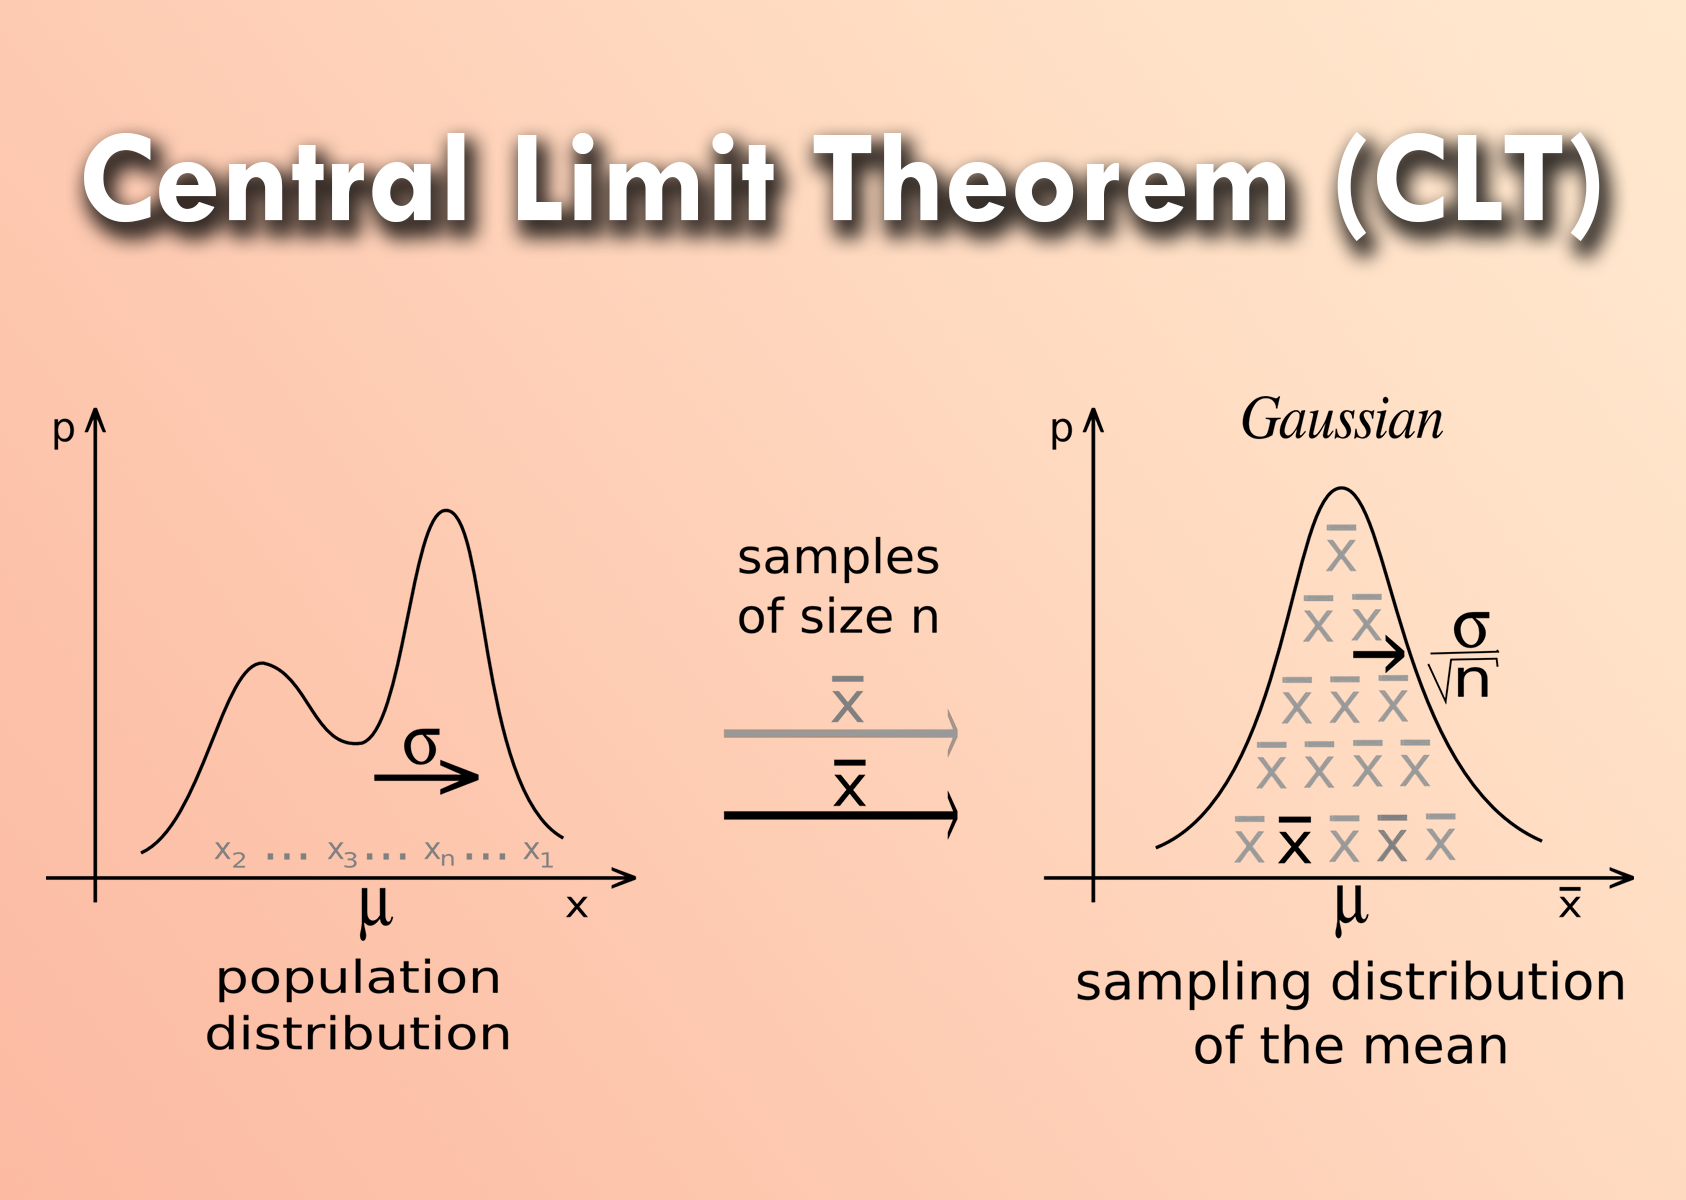
\includegraphics[width=\textwidth]{figures/clt.png}

\end{column}

\begin{column}{0.43\textwidth}

\vspace{0.6cm}

Regardless of the original population’s shape, the distribution of sample means becomes approximately Gaussian (normal) as sample size n increases. 

\vspace{0.4cm}

It is centered at the population mean $\mu$, with standard error $\frac{\sigma}{\sqrt n}$, showing that larger samples produce more precise estimates.

\end{column}

\end{columns}

\end{frame}

% ---------------------------------------------------------
% 30.2 CENTRAL LIMIT THEOREM -- APPLICATION
% ---------------------------------------------------------

\begin{frame}{30.2 Central Limit Theorem -- Application}

\textbf{Why is the CLT important?}

The CLT provides the theoretical basis for many statistical
procedures involving sample means.

\vspace{0.4cm}

It is used in:

\begin{itemize}
    \item Confidence interval construction
    \item Hypothesis testing
    \item Approximation of sampling distributions
    \item Statistical inference from large samples
\end{itemize}

\vspace{0.4cm}

\[
\boxed{
n\uparrow
\quad\Rightarrow\quad
SE(\bar{X})=\frac{\sigma}{\sqrt n}\downarrow
}
\]

\vspace{0.2cm}

Larger samples generally produce more stable estimates of
the population mean.

\end{frame}


% ---------------------------------------------------------
% 31. CONFIDENCE INTERVALS
% ---------------------------------------------------------

\begin{frame}{31. Confidence Intervals}

\textbf{Definition}

A confidence interval is an interval calculated from sample
data that provides a range of plausible values for an unknown
population parameter.

\vspace{0.4cm}

For a population mean with known $\sigma$, a confidence interval
can be written as:

\[
\boxed{
\bar{x}
\pm
z_{\alpha/2}
\frac{\sigma}{\sqrt n}
}
\]

where $z_{\alpha/2}$ is the appropriate standard normal
critical value.

\vspace{0.3cm}

\textbf{General form}

\[
\boxed{
\text{Estimate}
\pm
\text{Margin of Error}
}
\]

\end{frame}


% ---------------------------------------------------------
% 31.1 CONFIDENCE INTERVALS -- EXAMPLE
% ---------------------------------------------------------

\begin{frame}{31.1 Confidence Intervals -- Example}

\textbf{Example}

Suppose:
\[
\bar{x}=50,\qquad
\sigma=10,\qquad
n=100
\]

For a $95\%$ confidence interval:
\[
z_{0.025}=1.96
\]

The margin of error is
\[
1.96\frac{10}{\sqrt{100}}
=
1.96
\]

Therefore,
\[
CI
=
50\pm1.96
\]
\[
\boxed{
CI=(48.04,\;51.96)
}
\]
Using this procedure, the interval obtained from the sample is intended to capture the true population mean in the long-run at the stated confidence level.

\end{frame}


% ---------------------------------------------------------
% 31.2 CONFIDENCE INTERVALS -- KEY POINTS
% ---------------------------------------------------------

\begin{frame}{31.2 Confidence Intervals -- Key Points}

The width of a confidence interval depends on:

\begin{itemize}
    \item Sample size
    \item Variability of the data
    \item Chosen confidence level
\end{itemize}

For the mean:
\[
\boxed{
\text{Margin of Error}
=
z_{\alpha/2}
\frac{\sigma}{\sqrt n}
}
\]

\textbf{Effect of sample size}

\[
n\uparrow
\quad\Rightarrow\quad
\frac{\sigma}{\sqrt n}\downarrow
\]

Therefore, larger samples generally lead to
\textbf{narrower confidence intervals}.

\end{frame}
% =========================================================
% PART V -- MODEL ESTIMATION
% =========================================================

\section{Model Estimation}

% ---------------------------------------------------------
% 32. PARAMETRIC MODEL ESTIMATION
% ---------------------------------------------------------

\begin{frame}{32. Parametric Model Estimation}

\textbf{Definition}

Parametric model estimation assumes that the population
distribution belongs to a known family of distributions
described by a finite number of parameters.

\textbf{Examples}

\begin{itemize}
    \item Normal distribution -- parameters $\mu$ and $\sigma^2$
    \item Bernoulli distribution -- parameter $p$
    \item Poisson distribution -- parameter $\lambda$
\end{itemize}

\vspace{0.1cm}

A parametric model can be written as
\[
\boxed{
f(x;\theta)
}
\]

where $\theta$ represents the unknown parameter(s).

\textbf{Goal}

Estimate the unknown parameters using observed sample data.

\end{frame}


% ---------------------------------------------------------
% 32.1 PARAMETRIC MODEL -- EXAMPLE
% ---------------------------------------------------------

\begin{frame}{32.1 Parametric Model Estimation -- Example}

\textbf{Example}

Suppose a population is assumed to follow a normal distribution:
\[
X\sim N(\mu,\sigma^2)
\]

The parameters are:
\[
\mu=\text{population mean}
\]
\[
\sigma^2=\text{population variance}
\]

Given a sample, we can estimate these parameters using:
\[
\hat{\mu}=\bar{x}
\]

\[
\hat{\sigma}^2=s^2
\]

The assumed distribution provides a mathematical model, while
the sample data is used to estimate its unknown parameters.

\end{frame}


% ---------------------------------------------------------
% 33. MAXIMUM LIKELIHOOD ESTIMATION
% ---------------------------------------------------------

\begin{frame}{33. Maximum Likelihood Estimation}

\textbf{Definition}

Maximum Likelihood Estimation (MLE) is a method for estimating
unknown parameters by choosing the parameter values that make
the observed data most likely.

For observations
\[
x_1,x_2,\ldots,x_n
\]

the likelihood function is
\[
\boxed{
L(\theta)
=
\prod_{i=1}^{n}f(x_i;\theta)
}
\]

The maximum likelihood estimator is
\[
\boxed{
\hat{\theta}
=
\arg\max_{\theta}L(\theta)
}
\]

Choose the parameter value that gives the highest likelihood
for the observed data.

\end{frame}


% ---------------------------------------------------------
% 33.1 MLE -- LOG-LIKELIHOOD
% ---------------------------------------------------------

\begin{frame}{33.1 Maximum Likelihood Estimation -- Log-Likelihood}

Since likelihoods involve products, it is often easier to
maximize the logarithm of the likelihood.

The log-likelihood is
\[
\boxed{
\ell(\theta)=\log L(\theta)
}
\]

Therefore,
\[
\boxed{
\hat{\theta}
=
\arg\max_{\theta}\ell(\theta)
}
\]

Because the logarithm is a monotonically increasing function,
\[
\arg\max_{\theta}L(\theta)
=
\arg\max_{\theta}\log L(\theta)
\]

\textbf{Advantage}

The logarithm converts products into sums, making
mathematical calculations easier.

\end{frame}


% ---------------------------------------------------------
% 33.2 MLE -- SIMPLE EXAMPLE
% ---------------------------------------------------------

\begin{frame}{33.2 Maximum Likelihood Estimation -- Example}

\textbf{Example: Bernoulli Distribution}

Let
\[
X\in\{0,1\}, \qquad P(X=x)=p^x(1-p)^{1-x}
\]

where $p$ is the unknown probability of success.

For observations $x_1,\ldots,x_n$, the likelihood is
\[
L(p)=\prod_{i=1}^{n}p^{x_i}(1-p)^{1-x_i}
\]

The MLE is obtained by maximizing $L(p)$:
\[
\boxed{\hat{p}=\frac{1}{n}\sum_{i=1}^{n}x_i}
\]

$\hat p$ is the \textbf{sample proportion of successes}.

\end{frame}


% ---------------------------------------------------------
% 34. NON-PARAMETRIC MODEL ESTIMATION
% ---------------------------------------------------------

\begin{frame}{34. Non-parametric Model Estimation}

\textbf{Definition}

Non-parametric model estimation does not assume that the
population distribution belongs to a specific parametric family.

Instead, the distribution is estimated directly from the
observed data.

\textbf{Examples}

\begin{itemize}
    \item Empirical Cumulative Distribution Function (ECDF)
    \item Kernel Density Estimation (KDE)
\end{itemize}

\textbf{Key idea}
\[
\boxed{
\text{Data}
\longrightarrow
\text{Estimate Distribution}
}
\]
without requiring a fixed distribution such as normal,
Poisson, or Bernoulli.

\textbf{Advantage}

Flexible when the underlying distribution is unknown or
does not fit a simple parametric family.

\end{frame}


% ---------------------------------------------------------
% 35. EMPIRICAL CDF
% ---------------------------------------------------------

\begin{frame}{35. Empirical CDF}

\textbf{Definition}

The Empirical Cumulative Distribution Function (ECDF) estimates
the cumulative distribution function directly from sample data.

\vspace{0.4cm}

For a sample
\[
x_1,x_2,\ldots,x_n,
\]

the empirical CDF is
\[
\boxed{
F_n(x)
=
\frac{1}{n}
\sum_{i=1}^{n}
\mathbf{1}(x_i\leq x)
}
\]

where $\mathbf{1}(\cdot)$ is the indicator function.

\textbf{Interpretation}

$F_n(x)$ represents the proportion of sample observations
that are less than or equal to $x$.

\end{frame}


% ---------------------------------------------------------
% 35.1 EMPIRICAL CDF -- EXAMPLE
% ---------------------------------------------------------

\begin{frame}{35.1 Empirical CDF -- Example}

Consider the ordered sample:
\[
X=\{10,20,30,40,50\}
\]
Since $n=5$:
\[
F_n(x)
=
\frac{\text{Number of observations}\leq x}{5}
\]

\begin{columns}[T]

\begin{column}{0.48\textwidth}

\[
F_n(30)=0.6
\]

This means that $60\%$ of the observations
are less than or equal to $30$.

\end{column}

\begin{column}{0.48\textwidth}

\begin{table}
\centering
\small

\begin{tabular}{c c}
\toprule
$x$ & $F_n(x)$ \\
\midrule
10 & $1/5=0.2$ \\
20 & $2/5=0.4$ \\
30 & $3/5=0.6$ \\
40 & $4/5=0.8$ \\
50 & $5/5=1.0$ \\
\bottomrule
\end{tabular}

\end{table}

\end{column}

\end{columns}

\end{frame}


% ---------------------------------------------------------
% 36. KERNEL DENSITY ESTIMATION
% ---------------------------------------------------------

\begin{frame}{36. Kernel Density Estimation}

\textbf{Definition}

Kernel Density Estimation (KDE) is a non-parametric method
for estimating the probability density function of a dataset.

\vspace{0.4cm}

For observations $x_1,\ldots,x_n$:

\[
\boxed{
\hat{f}_h(x)
=
\frac{1}{nh}
\sum_{i=1}^{n}
K\left(
\frac{x-x_i}{h}
\right)
}
\]

where:

\begin{itemize}
    \item $K$ = kernel function
    \item $h$ = bandwidth
    \item $n$ = number of observations
\end{itemize}

\end{frame}


% ---------------------------------------------------------
% 36.1 KDE -- BANDWIDTH
% ---------------------------------------------------------

\begin{frame}{36.1 Kernel Density Estimation -- Bandwidth}

The \textbf{bandwidth} $h$ controls the smoothness of the
estimated density.

\textbf{Small bandwidth}

\[
h\downarrow
\quad\Rightarrow\quad
\text{More detailed / less smooth estimate}
\]

\textbf{Large bandwidth}

\[
h\uparrow
\quad\Rightarrow\quad
\text{Smoother estimate}
\]

\textbf{Key idea}

The bandwidth determines how much neighboring observations
influence the estimated density.

\textbf{Application}

KDE is useful for visualizing and estimating unknown
continuous distributions.

\end{frame}


% ---------------------------------------------------------
% 36.2 KDE -- BASIC EXAMPLE
% ---------------------------------------------------------

\begin{frame}{36.2 Kernel Density Estimation -- Example}

\textbf{Example}

Consider the sample:

\[
X=\{2,3,3,4,5\}
\]

KDE places a small smooth kernel around each observation.

\vspace{0.4cm}

The individual kernels are combined to produce an estimated
density:

\[
\boxed{
\text{Individual Kernels}
\longrightarrow
\text{Combined Density Estimate}
}
\]

\vspace{0.4cm}

\textbf{Interpretation}

Instead of assuming that the data follows a normal distribution,
KDE estimates the shape of the distribution directly from the data.

\end{frame}

% ---------------------------------------------------------
% 36.3 KERNEL DENSITY ESTIMATION -- FIGURE
% ---------------------------------------------------------

\begin{frame}{36.3 Kernel Density Estimation -- Figure}

\begin{columns}[T]

\begin{column}{0.62\textwidth}

\centering
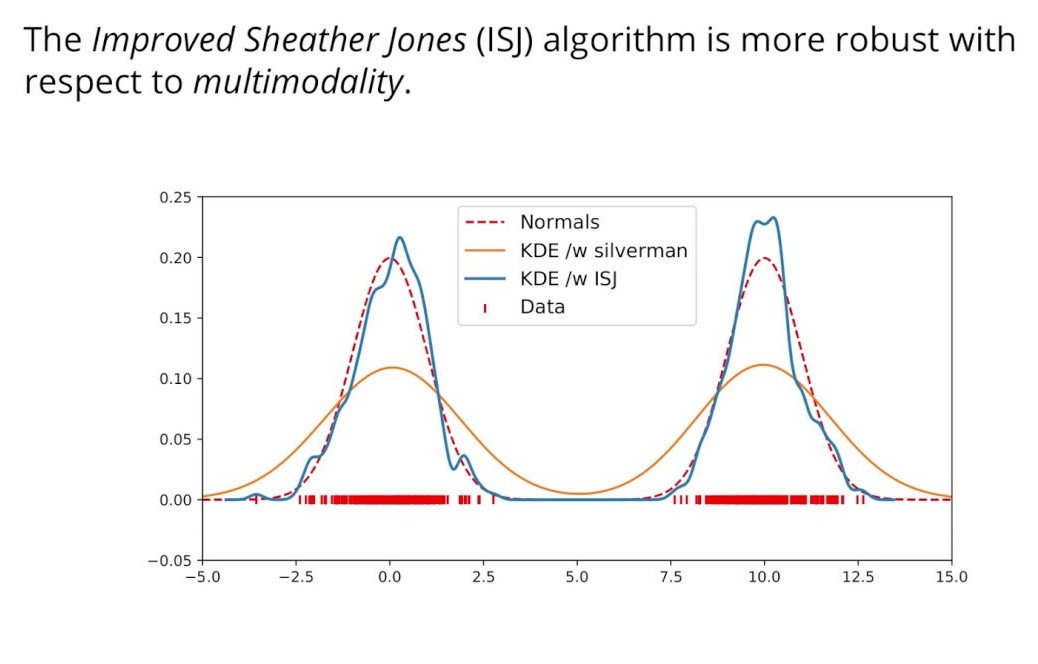
\includegraphics[width=\textwidth]{figures/kde.jpg}

\end{column}

\begin{column}{0.34\textwidth}

\vspace{0.8cm}

The figure shows a smooth density curve
estimated from observed data points.

\vspace{0.4cm}

Unlike a histogram, KDE produces a continuous
estimate of the underlying distribution.

\end{column}

\end{columns}

\end{frame}
% ---------------------------------------------------------
% 37. PARAMETRIC VS NON-PARAMETRIC
% ---------------------------------------------------------

\begin{frame}{37. Parametric vs Non-parametric Model Estimation}

\small

\begin{table}
\centering

\begin{tabular}{>{\bfseries}l l l}
\toprule
Feature & Parametric & Non-parametric \\
\midrule
Distribution assumption &
Specific family &
No fixed family \\

Parameters &
Finite number &
More flexible \\

Flexibility &
Lower &
Higher \\

Examples &
Normal, Poisson &
ECDF, KDE \\

Data requirement &
Often fewer observations &
Often more data needed \\

\bottomrule
\end{tabular}

\end{table}

\vspace{0.4cm}

\textbf{Key idea}

\[
\boxed{
\text{Parametric}
\rightarrow
\text{Assume a distribution}
}
\]

\[
\boxed{
\text{Non-parametric}
\rightarrow
\text{Estimate from data}
}
\]

\end{frame}


% ---------------------------------------------------------
% 37.1 PARAMETRIC VS NON-PARAMETRIC -- APPLICATION
% ---------------------------------------------------------

\begin{frame}{37.1 Parametric vs Non-parametric -- Application}

\textbf{Parametric estimation}

Useful when a suitable probability distribution can reasonably
describe the data.

\vspace{0.1cm}

\textbf{Non-parametric estimation}

Useful when the underlying distribution is unknown,
irregular, or difficult to represent using a simple
parametric model.

\vspace{0.1cm}

\textbf{In AI and Data Science}

The choice depends on:

\begin{itemize}
    \item Amount of available data
    \item Distributional assumptions
    \item Required flexibility
    \item Computational cost
    \item Purpose of the analysis
\end{itemize}

\vspace{0.1cm}

\end{frame}
% =========================================================
% 08 - APPLICATIONS, CONCLUSION AND THANK YOU
% =========================================================

\section{Applications and Conclusion}

% ---------------------------------------------------------
% 38. APPLICATIONS IN COMPUTING AND AI
% ---------------------------------------------------------

\begin{frame}{38. Applications in Computing and AI}

Descriptive statistics provides a foundation for understanding
and analyzing data in computing and Artificial Intelligence.

\vspace{0.3cm}

\begin{itemize}

    \item \textbf{Data Analysis}
    \begin{itemize}
        \item Summarizes large datasets using mean, median, variance and other measures.
    \end{itemize}

    \item \textbf{Data Preprocessing}
    \begin{itemize}
        \item Histograms and box plots help identify distributions and potential outliers.
    \end{itemize}

    \item \textbf{Feature Analysis}
    \begin{itemize}
        \item Covariance and correlation help study relationships between variables.
    \end{itemize}

    \item \textbf{Machine Learning}
    \begin{itemize}
        \item Statistical concepts support model estimation, evaluation and uncertainty analysis.
    \end{itemize}

    \item \textbf{AI Applications}
    \begin{itemize}
        \item Used in areas such as prediction, classification, anomaly detection and pattern analysis.
    \end{itemize}

\end{itemize}

\end{frame}


% ---------------------------------------------------------
% 39. CONCLUSION
% ---------------------------------------------------------

\begin{frame}{39. Conclusion}

\begin{itemize}

    \item Descriptive statistics provides systematic methods for
    summarizing and understanding data.

    \item Measures of central tendency describe the typical value
    of a dataset.

    \item Measures of dispersion describe the variability of data.

    \item Graphical methods such as histograms and box plots
    provide visual understanding of distributions and outliers.

    \item Covariance and correlation help identify relationships
    between variables.

    \item Frequentist concepts provide a foundation for
    sampling, estimation and statistical inference.

    \item Parametric and non-parametric methods provide different
    approaches for estimating underlying data distributions.

    \item These concepts form an important mathematical foundation
    for data science, machine learning and Artificial Intelligence.

\end{itemize}

\end{frame}

% ---------------------------------------------------------
% REFERENCES
% ---------------------------------------------------------

\nocite{*}

\begin{frame}[allowframebreaks]{References}

\bibliographystyle{plain}
\bibliography{references/references}

\end{frame}
% =========================================================

\section{Thank You}
% ---------------------------------------------------------
% THANK YOU
% ---------------------------------------------------------

\begin{frame}

\centering

\vspace{1.5cm}

{\Huge \textbf{Thank You}}

\vfill

{\normalsize Arya T S}

\end{frame}

\end{document}